%% Chapter 5 — Kubernetes
\setcounter{chapter}{4}
\chapter{Kubernetes}
\chaptersubtitle{A control loop for your serving fleet — desired state, honest budgets, and a scheduler for expensive metal}

\begin{calloutbox}{tbbblue}{tbbbluefill}
{\normalsize\bfseries\color{tbbblue}Learning objectives}\par\vspace{3pt}
\begin{tbbitemize}
  \item Explain Kubernetes's one core idea — desired state in a database, reconciled by control loops — and predict what the cluster does when reality drifts: a pod dies, a node vanishes, a deploy changes the spec.
  \item Name the control-plane and node components, and trace one \code{kubectl apply} end to end: API server → etcd → controllers → scheduler → kubelet → containerd/runc → Chapter 3's namespaces and cgroups.
  \item Deploy a model server as Pod + Deployment + Service; wire startup, readiness, and liveness probes correctly around a slow model load; and explain how readiness gates both traffic and rollouts.
  \item Translate resource requests and limits into what each actually is — scheduler arithmetic versus cgroup files — compute node packing by hand, and choose QoS classes for serving pods deliberately.
  \item Reason about GPU scheduling: extended resources and integer allocation, taints and affinity, bin-packing versus spreading, and the fragmentation that quietly strands the most expensive hardware in the fleet.
  \item Diagnose the six canonical pod failure states — Pending, ImagePullBackOff, CrashLoopBackOff, OOMKilled, Evicted, and ready-but-unrouted — from their signatures, with the right first command for each.
\end{tbbitemize}
\end{calloutbox}

\vspace{5.0pt}

\begin{calloutbox}{tbbteal}{tbbtealfill}
{\normalsize\bfseries\color{tbbteal}Key terms}\par\vspace{3pt}
control plane · API server · etcd · scheduler · controller manager · reconciliation · kubelet · CRI · monolith · microservice architecture (MSA) · pod · pause container · label / selector · Deployment · ReplicaSet · rolling update · Service · ClusterIP / NodePort / LoadBalancer · endpoints · kube-proxy · CoreDNS · startup / readiness / liveness probes · requests / limits · allocatable · overcommit · QoS class (Guaranteed / Burstable / BestEffort) · node-pressure eviction · taint / toleration · nodeSelector / affinity · extended resource · nvidia.com/gpu · device plugin · Pending · CrashLoopBackOff · OOMKilled · Evicted
\end{calloutbox}

\vspace{5.0pt}

\begin{calloutbox}{tbblightgray}{tbbboxfill}
{\normalsize\bfseries\color{tbbink}Chapter outline}\par\vspace{3pt}
\textbf{5.1} The cluster as a control loop    \textbf{5.2} Anatomy: a database with opinions    \textbf{5.3} Pods, Deployments, Services — the serving trinity    \textbf{5.4} requests, limits, and QoS: Chapter 3 at fleet scale    \textbf{5.5} GPUs and the scheduler    \textbf{5.6} A field guide to dying pods    \textbf{5.7} Lab: your model server, orchestrated — followed by a summary, exercises, and further reading.
\end{calloutbox}

\vspace{3.0pt}

\begin{calloutbox}{tbbamber}{tbbamberfill}
{\normalsize\bfseries\color{tbbamberdark}How to read this chapter}\par\vspace{3pt}
Like Chapter 3, this chapter is written to be \textbf{read next to a terminal}. Every transcript reproduces on a laptop cluster — \code{minikube start} (or kind) is the only prerequisite — except the GPU transcripts, which are shown against a managed GPU node pool: the commands are identical, only the hardware differs. The YAML files are in the course repository, but typing them once is worth more than cloning them.
\end{calloutbox}

\section{The Cluster as a Control Loop}

Chapter 4 ended with a satisfying artifact: your model server, packaged into an image, pushed to a registry, GPU access understood down to the device plugin. One \code{docker run} on one VM and you are serving. For a demo, that is the end of the story. Then Chapter 1's actual requirements show up, all at once: you need \textbf{many replicas} — for throughput, and so one crash is not an outage; you need \textbf{deploys that drop nothing} (Chapter 3's SIGTERM tape, now playing weekly); you need to survive a \textbf{node dying at 3 a.m.} without a human awake; you are running \textbf{twenty models} with different hardware needs on a shared bill; and the GPUs — the most expensive line in that bill — must never sit idle merely because a human forgot to place work on them.

You could script all of this. Everyone did, circa 2014: a bash loop over SSH, a cron job that curls health endpoints and restarts what fails, a wiki page describing which model runs where. Grow those scripts honestly and they converge on a shape: \textbf{a file describing what should be running, a loop comparing that file to what is running, and actions that close the gap.} Kubernetes is that shape, industrialized — descended from Google's internal Borg system, which ran on exactly this idea for a decade before Kubernetes brought it outside. Understand the shape and the rest of the chapter is detail.

\subsection*{The experiment that teaches the whole system}

Start with a running cluster (the lab walks through \code{minikube start}) on which a Deployment asks for three replicas of a model server. Now do something that would be sabotage anywhere else — kill one, and immediately look again:

\begin{terminalbox}
\begin{Verbatim}[breaklines=true,breakanywhere=true,fontsize=\small,formatcom=\color{tbbtermfg},codes=\tbbcodeactive]
$ kubectl get pods
NAME                            READY   STATUS    RESTARTS   AGE
model-server-7d4b9c6f5-8xk2p    1/1     Running   0          2d
model-server-7d4b9c6f5-tq9wz    1/1     Running   0          2d
model-server-7d4b9c6f5-zl6vn    1/1     Running   0          2d
$ kubectl delete pod model-server-7d4b9c6f5-zl6vn   # sabotage
pod "model-server-7d4b9c6f5-zl6vn" deleted
$ kubectl get pods
NAME                            READY   STATUS    RESTARTS   AGE
model-server-7d4b9c6f5-8xk2p    1/1     Running   0          2d
model-server-7d4b9c6f5-tq9wz    1/1     Running   0          2d
model-server-7d4b9c6f5-fh5m8    1/1     Running   0          4s
\end{Verbatim}
\end{terminalbox}
\figcaption{Transcript 5-1  Delete a pod; four seconds later a new one exists (note the new name suffix and AGE). Nobody restarted anything — a controller noticed that 2 did not equal 3.}

Read the last line carefully: a \textbf{new} pod — different suffix, four seconds old — not your old pod resurrected. You did not restart anything; more precisely, \textbf{you never asked for pods at all.} You declared a Deployment whose spec says \code{replicas: 3}, and a controller — a loop that runs forever comparing desired to actual — observed 2 ≠ 3 and created one. Your deletion was not an event anyone handled; it was \textbf{drift}, and drift gets corrected (Figure 5-1). This is why the grammar of Kubernetes feels strange at first: you write \textbf{nouns} (objects: "a Deployment with three replicas"), never verbs. The verbs — create, restart, reschedule — are emergent, performed by controllers on your nouns' behalf.

\begin{tbbfigure}
  \adjustbox{max width=0.94\linewidth,max totalheight=0.46\textheight}{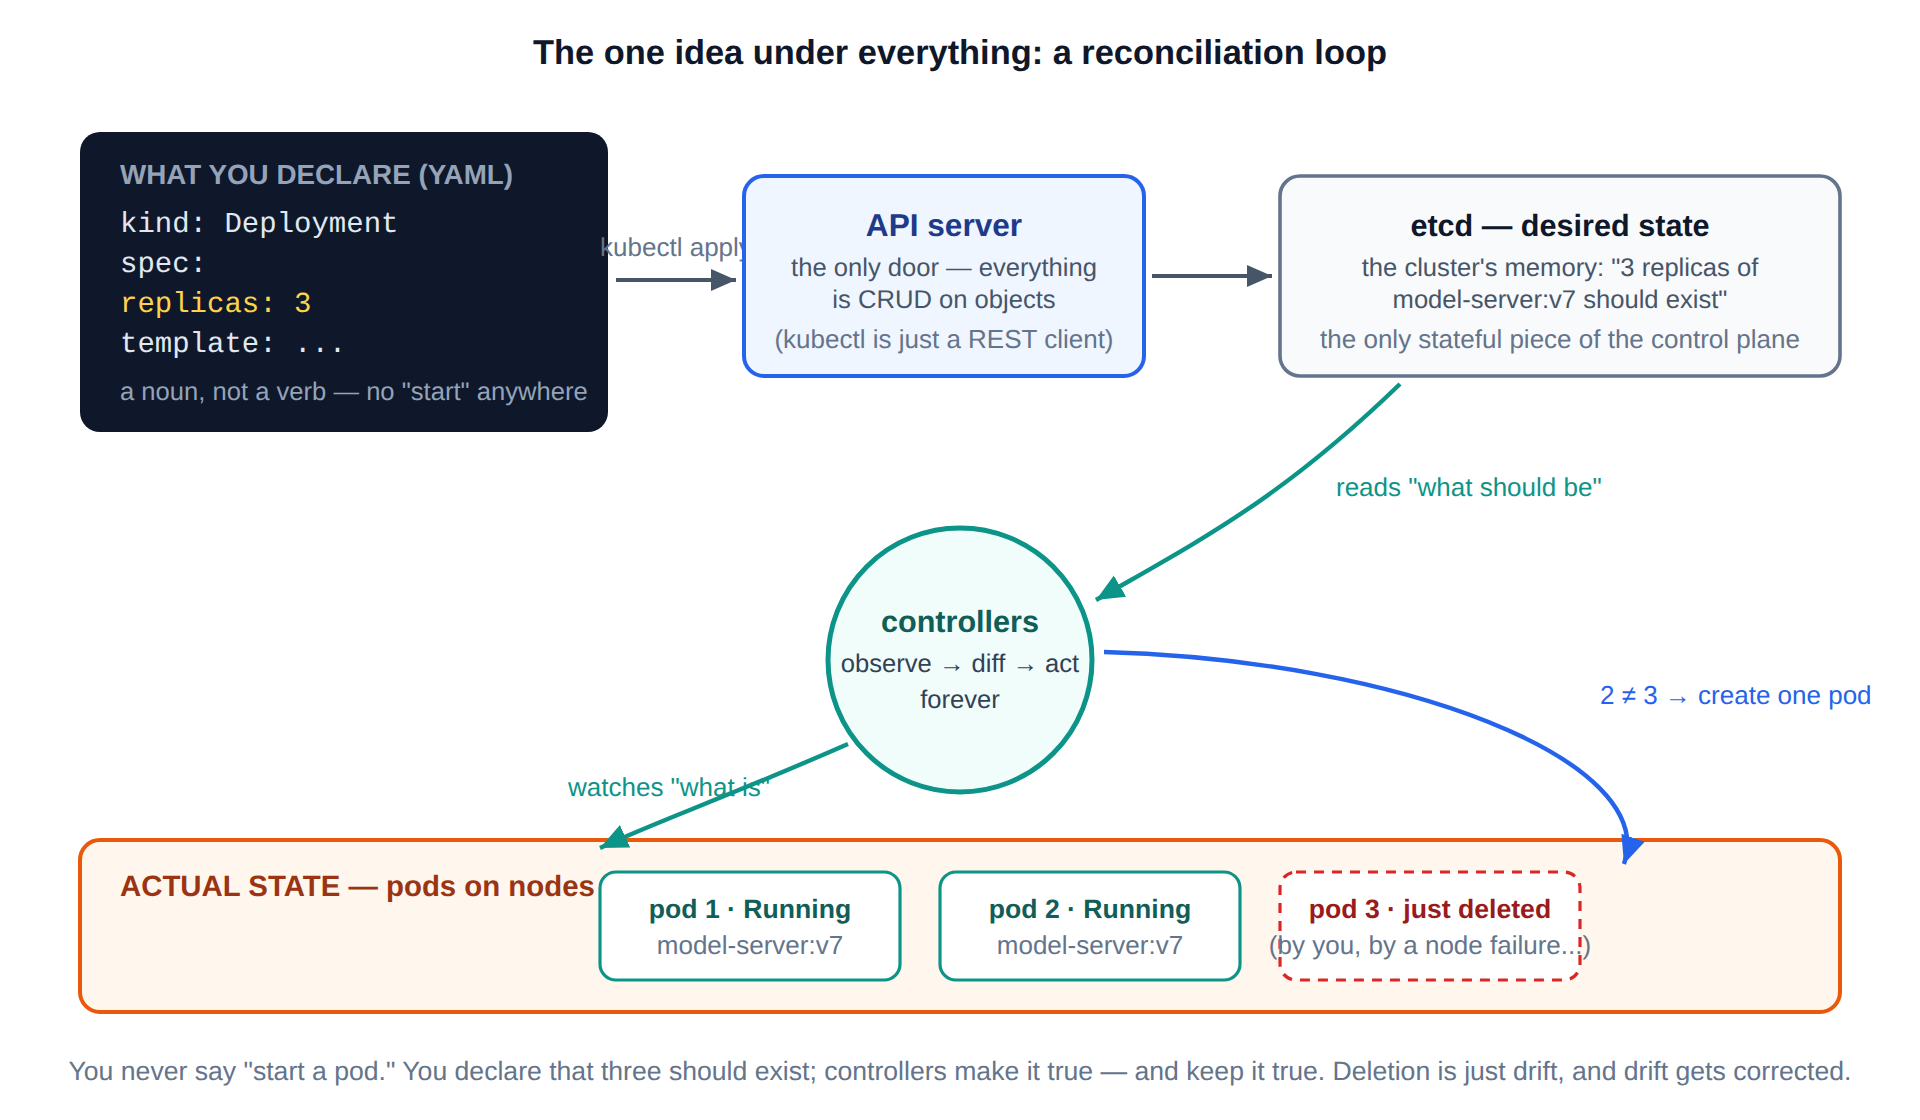
\includegraphics{figures/fig5-1_loop.png}}\\[3pt]
  \figcaption{Figure 5-1  The reconciliation loop. Desired state lives in etcd behind the API server; controllers watch both sides and act to close any gap — forever.}
\end{tbbfigure}

\subsection*{Declarative beats imperative at 3 a.m.}

The distinction has a name. An \textbf{imperative} system takes instructions: "start three servers." An instruction executes once, and its correctness decays: if a server dies later, the instruction is long gone; someone must notice and issue a new one. A \textbf{declarative} system holds an \textit{invariant}: "three servers exist." An invariant does not decay — it is re-checked and re-enforced continuously, which means the answer to "what happens when X fails?" is always the same: \textit{the loop notices and converges again}. A thermostat is the household version: you declare 21°C, and you do not re-issue the declaration when someone opens a window. This property is precisely what a serving fleet needs, because the 3 a.m. node failure, the fat-fingered deletion, and the deploy that halves the fleet are all, to the loop, the same thing: drift.

The declarative habit also pays compound interest later in this course. When Week 12 adds autoscaling, the autoscaler will not be a new kind of machinery — it is just \textbf{another writer of desired state}, editing \code{replicas: 3} to \code{replicas: 7} under load and letting this section's loop do everything else. When Week 13 automates deploys with CI/CD, the pipeline's final act is a one-line change to an object. Everything in the operations half of this course is someone or something editing nouns; the loop of Figure 5-1 is the only engine.

\subsection*{What this chapter is really about}

For a serving engineer, Kubernetes matters at four altitudes, and the chapter visits each. At the top, the \textbf{control loop} (this section) explains the system's behavior under every failure you will meet. One level down, the \textbf{objects} — Pod, Deployment, Service (§5.3) — are the vocabulary in which your model server is described, health-checked, and given a stable address. Below that, \textbf{resources and QoS} (§5.4) are where Chapter 3's cgroup walls get ghostwritten at fleet scale — including the OOM behavior you can now narrate in your sleep. And at the bottom, the \textbf{scheduler} (§5.5) decides which expensive GPU runs which model — a placement problem with a monthly price tag. Section 5.6 then turns the whole stack into what it becomes on the job: a diagnostic discipline.

\begin{calloutbox}{tbbpurple}{tbbpurplefill}
{\normalsize\bfseries\color{tbbpurple}Think About It}\par\vspace{3pt}
\begin{tbbitemize}
  \item The controller saw 2 ≠ 3 and created a pod. Suppose you instead manually create a fourth pod carrying the same labels the ReplicaSet selects on. What must the controller do, and what does that imply about how membership is decided?
  \item Why is a reconciliation loop more robust to the controller itself crashing than an imperative script is to the script host crashing? (Hint: what state does each need to resume correctly?)
  \item In Week 12, the Horizontal Pod Autoscaler will react to load by changing one integer in one object. List everything this section says must then happen automatically — and notice how little the autoscaler itself has to know.
\end{tbbitemize}
\end{calloutbox}

\section{Anatomy: A Database With Opinions}

Strip the mystique and Kubernetes has a one-sentence architecture: \textbf{a database (etcd) with an API in front (the API server) and a swarm of control loops behind (controllers, the scheduler, and one kubelet per node).} Everything else is commentary. Figure 5-2 lays the pieces out; this section gives each one its paragraph, then traces a single \code{kubectl apply} through all of them — because the chain, not the parts, is what you will debug.

\begin{tbbfigure}
  \adjustbox{max width=0.94\linewidth,max totalheight=0.46\textheight}{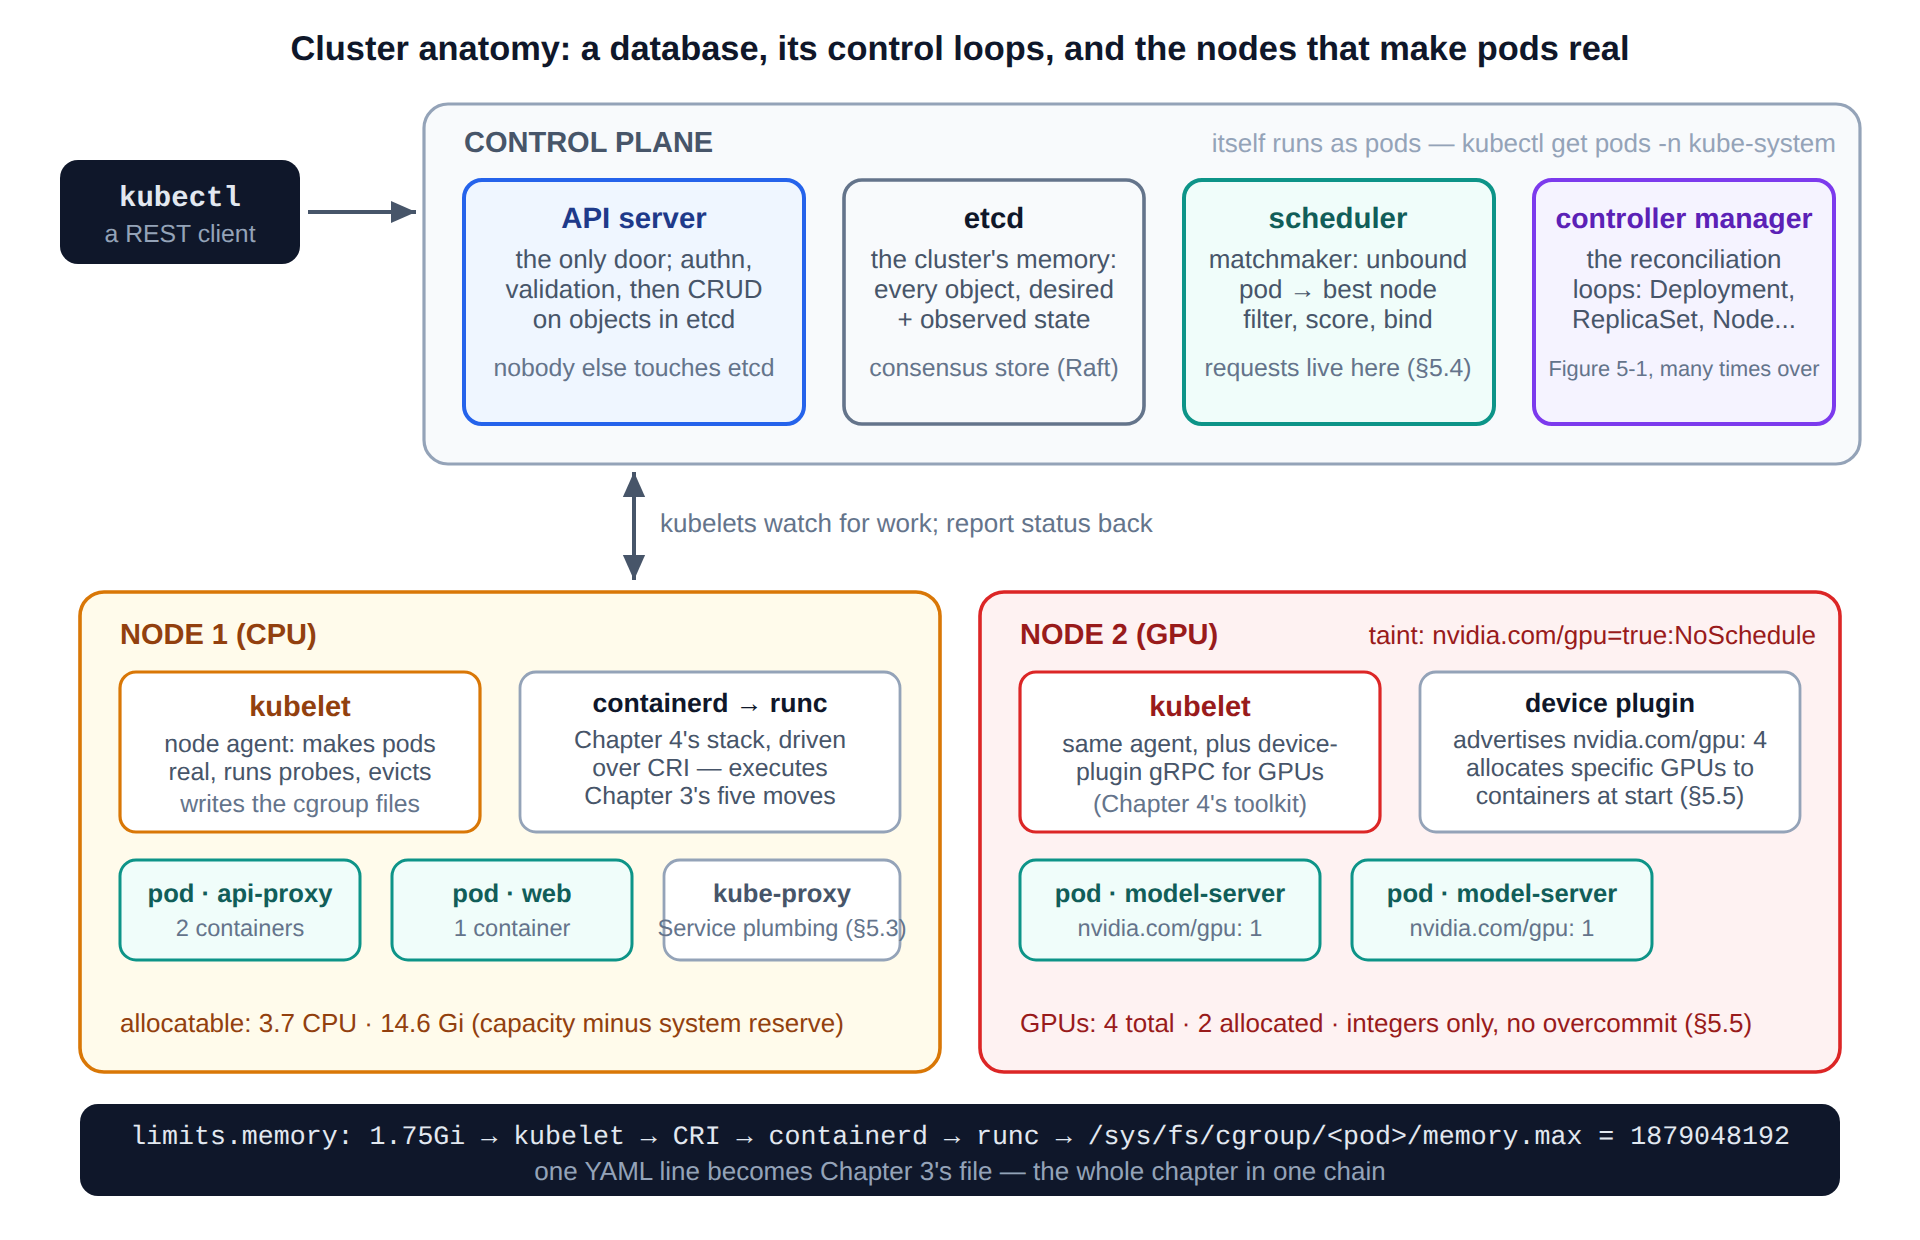
\includegraphics{figures/fig5-2_architecture.png}}\\[3pt]
  \figcaption{Figure 5-2  Cluster anatomy. The control plane stores and reconciles desired state; each node's kubelet makes pods real through Chapter 4's runtime stack — ending at Chapter 3's namespaces and cgroups.}
\end{tbbfigure}

\subsection*{The control plane, one paragraph per part}

The \textbf{API server} is the only door. Every actor — you via kubectl, every controller, every kubelet — talks to it and only to it; nothing else is allowed to touch etcd. It authenticates, authorizes, validates, and then does something almost anticlimactic: CRUD on objects. There is no hidden orchestration brain inside it. Even \code{kubectl} is revealed, at higher verbosity, to be a thin REST client:

\begin{terminalbox}
\begin{Verbatim}[breaklines=true,breakanywhere=true,fontsize=\small,formatcom=\color{tbbtermfg},codes=\tbbcodeactive]
$ kubectl get pods -v=8 2>&1 | grep -E "GET http"
GET https://192.168.49.2:8443/api/v1/namespaces/default/pods?limit=500
# kubectl get pods = one HTTP GET. kubectl is a REST client with manners.
$ kubectl get pods -n kube-system
NAME                               READY   STATUS    RESTARTS      AGE
etcd-minikube                      1/1     Running   0             9d
kube-apiserver-minikube            1/1     Running   0             9d
kube-controller-manager-minikube   1/1     Running   0             9d
kube-scheduler-minikube            1/1     Running   0             9d
coredns-5dd5756b68-mfqpx           1/1     Running   0             9d
kube-proxy-b47rl                   1/1     Running   0             9d
\end{Verbatim}
\end{terminalbox}
\figcaption{Transcript 5-2  Two demystifications: kubectl is HTTP, and the control plane itself runs as pods in the kube-system namespace — the machinery is managed by the machinery.}

\textbf{etcd} is the cluster's memory: a small, consistent (Raft-consensus) key-value store holding every object — desired state and last-observed status alike. It is the \textit{only} stateful piece; every other component can be killed and, on restart, rebuilds its working knowledge simply by watching the API server again. This is a design decision worth admiring for a moment: state concentrated in one replicated store, everything else stateless and disposable — the same shape you will be told to give your own serving systems.

The \textbf{scheduler} is a matchmaker with a narrow job description: it watches for pods that have no node assigned, chooses the best node for each (a filter-then-score pass that §5.5 dissects, because GPUs make it interesting), and writes the choice back into the pod object. That is all — it starts nothing and touches no node. The \textbf{controller manager} hosts the reconciliation loops of §5.1 — the Deployment controller, the ReplicaSet controller, the node-lifecycle controller that notices dead nodes, and dozens more, each a small "observe, diff, act" loop over one object type.

On every node, the \textbf{kubelet} is the hands. It watches the API server for pods bound to \textit{its} node and makes them real: instructs the container runtime over CRI — the gRPC interface in front of Chapter 4's containerd → runc stack — mounts volumes, runs the probes of §5.3, reports status back, and under memory pressure performs the evictions of §5.4. Note who this makes the kubelet: \textbf{the ghostwriter Chapter 3 kept promising.} When a pod declares \code{limits.memory: 1.75Gi}, it is the kubelet, via the runtime, that causes \code{1879048192} to appear in a \code{memory.max} file. Alongside it runs \textbf{kube-proxy}, which programs the Service NAT of §5.3, and — on GPU nodes — the \textbf{device plugin} from Chapter 4, which tells the kubelet how many GPUs exist and which ones are free.

\subsection*{One apply, end to end}

Now run the chain. You type \code{kubectl apply -f deployment.yaml} for a new three-replica model server. In order, and with nobody in charge:

\begin{tbbitemize}
  \item \textbf{1 — Persist.} The API server validates the Deployment object and writes it to etcd. Nothing is running; a row changed in a database.
  \item \textbf{2 — Expand.} The Deployment controller notices a Deployment with no matching ReplicaSet and creates one (an object, again). The ReplicaSet controller notices desired 3, actual 0, and creates three Pod objects — each with an empty \code{nodeName}.
  \item \textbf{3 — Place.} The scheduler notices three unbound pods, runs its filter-and-score pass per pod, and writes a node name into each. Still nothing has executed anywhere.
  \item \textbf{4 — Realize.} Each chosen node's kubelet sees a pod bound to it, pulls the image if absent (Chapter 3's 25–60 s cold-pull arithmetic applies here, per node), and drives containerd → runc to create the pause container and your server container — unshared namespaces, cgroup files written, overlayfs mounted: Chapter 3's five moves, performed by machinery.
  \item \textbf{5 — Report.} The kubelet posts status back; probes begin; when readiness passes, the pod's IP joins the Service endpoints (§5.3) and traffic flows.
\end{tbbitemize}

Two things about this chain deserve italics. First, \textit{nothing named Kubernetes ran your container} — runc did; Kubernetes decided where and kept score. If Chapter 3 demystified the container, this section demystifies the orchestrator: it is bookkeeping around the same kernel mechanisms. Second, \textit{every arrow in the chain is a watch on the API server} — components never call each other. That radical decoupling is why the system tolerates any single piece being down: the work waits in etcd, and whoever resumes picks it up. (It also means the data plane keeps serving when the control plane is sick: already-running pods, already-programmed Service routes, and already-written cgroup files need no permission to keep working — you merely cannot \textit{change} anything until the control plane returns.)

\begin{calloutbox}{tbbpurple}{tbbpurplefill}
{\normalsize\bfseries\color{tbbpurple}Think About It}\par\vspace{3pt}
\begin{tbbitemize}
  \item etcd loses quorum for ten minutes. Which of these still work, and why: (a) existing pods serving traffic, (b) Service routing to them, (c) a rolling update, (d) self-healing after a pod crash?
  \item Why does the architecture forbid components from talking to each other directly (scheduler → kubelet, say) instead of through watches on the API server? Name two failure scenarios this indirection absorbs.
  \item A controller crashes and restarts five minutes later. Explain why "level-triggered" reconciliation (act on observed state) survives this gracefully where "edge-triggered" (act on events) would not.
\end{tbbitemize}
\end{calloutbox}

\section{Pods, Deployments, Services — the Serving Trinity}

Three objects carry essentially every serving workload you will run in this course. The \textbf{Pod} is the unit of execution — your server plus its helpers. The \textbf{Deployment} is the fleet manager — how many, which version, how upgrades roll. The \textbf{Service} is the stable address — one name in front of mortal replicas. Learn these three deeply and most Kubernetes YAML you meet is a variation.

\subsection*{First, a word about workload shape: microservices, briefly}

Before dissecting the three objects, it is worth naming the architectural style they quietly assume. The traditional alternative is the \textbf{monolith}: one deployable unit containing every capability — UI, business logic, data access — built from one codebase, released as one artifact, and scaled by running more copies of the whole thing. A \textbf{microservice architecture (MSA)} decomposes that application into small, independently deployable services, each owning a single capability (and, ideally, its own data), exposing it to the others only through a network API — HTTP or gRPC — and evolving on its own release cadence, usually under its own team.

The industry did not migrate for fashion; the wins are operational. \textbf{Independent deploys}: ship the recommender daily without re-releasing checkout. \textbf{Independent scaling}: add replicas only where the load is — and, in ML systems, only where the GPUs are. \textbf{Failure isolation}: a crashed recommendation service degrades a page; it does not take payments down. \textbf{Organizational fit}: small teams own small services end to end. The price is equally real, and it is the honest half of the story: every in-process function call becomes a \textbf{network call} — with latency, timeouts, partial failure, and distributed debugging attached — and one deployable becomes \textbf{N deployables}, each of which must be built, versioned, discovered, health-checked, scaled, and monitored.

\begin{calloutbox}{tbbteal}{tbbtealfill}
{\normalsize\bfseries\color{tbbteal}Monolith vs. microservices — the trade, compressed}\par\vspace{3pt}
\begin{tbbitemize}
  \item \textbf{Deploy} — monolith: one artifact, all-or-nothing releases. MSA: per-service releases on independent cadences.
  \item \textbf{Scale} — monolith: copy the whole thing. MSA: scale only the hot path (for serving: only the GPU-hungry part).
  \item \textbf{Failure} — monolith: shared fate. MSA: isolated blast radius — provided timeouts and fallbacks are actually designed (they are not free).
  \item \textbf{Calls} — monolith: in-process, nanoseconds. MSA: over the network — latency, partial failure, and tracing to reconstruct what happened.
  \item \textbf{Organization} — monolith: one codebase, coordination by meeting. MSA: team-per-service (Conway's law, used deliberately).
\end{tbbitemize}

The trade in one line: \textbf{code complexity is exchanged for operational complexity — and Kubernetes is where the industry standardized the operational half.}
\end{calloutbox}

\vspace{3.0pt}

That last line explains this chapter's existence. The operational burden MSA creates is nearly identical for every adopter — which made it industrializable, and Kubernetes is that industrialization. Read the trinity below as the \textbf{microservice starter kit}: a unit of deployment (the Pod), a fleet manager per service (the Deployment), and discovery with load balancing (the Service, one DNS name per service). And note that you never really chose the style: \textbf{an AI serving system is born a small MSA} — a CPU-cheap API gateway at the front (many small replicas, released weekly), one GPU-expensive model server per model behind it (few replicas, redeployed at every model version — Week 13), plus an entourage of pre/post-processors and exporters, each scaled to its own bottleneck. Different hardware, different scaling, different cadence: precisely the conditions microservices exist for. One rule of thumb will carry you through the rest of the course: \textbf{one microservice = one Deployment + one Service.} Week 9's serving frameworks assume it ("model-as-a-service"), Week 12's KServe formalizes it, and Week 14's observability stack exists because of it.

\subsection*{Pod: the unit of scheduling — and of sharing}

A pod is one or more containers that are scheduled as a unit and share two things: a \textbf{network identity} and \textbf{volumes}. Kubernetes implements the sharing with a trick you already know from Chapter 3: a tiny \textbf{pause container} is started first and \textit{owns the pod's NET namespace} (and IPC); your containers are then started joined to it (Figure 5-3). One pod, one IP; containers inside reach each other over \code{localhost}; their MNT and PID namespaces stay private, à la carte, exactly as §3.2 promised. The pause container is also why a pod survives your app container restarting: the network identity is held by a process that never crashes because it does nothing.

Why pods rather than bare containers? Because real servers have entourage: a metrics exporter, a log shipper, later a service-mesh proxy (Week 14 meets two of these). The pod is the "things that must live, die, and be scheduled together" boundary. The serving rule of thumb: \textbf{one main container per pod, sidecars only for cross-cutting plumbing} — never two model servers in one pod (they could not be scaled, upgraded, or OOM-isolated independently; and per Chapter 3, memory.max is per-container anyway, so the isolation is real).

\begin{tbbfigure}
  \adjustbox{max width=0.94\linewidth,max totalheight=0.46\textheight}{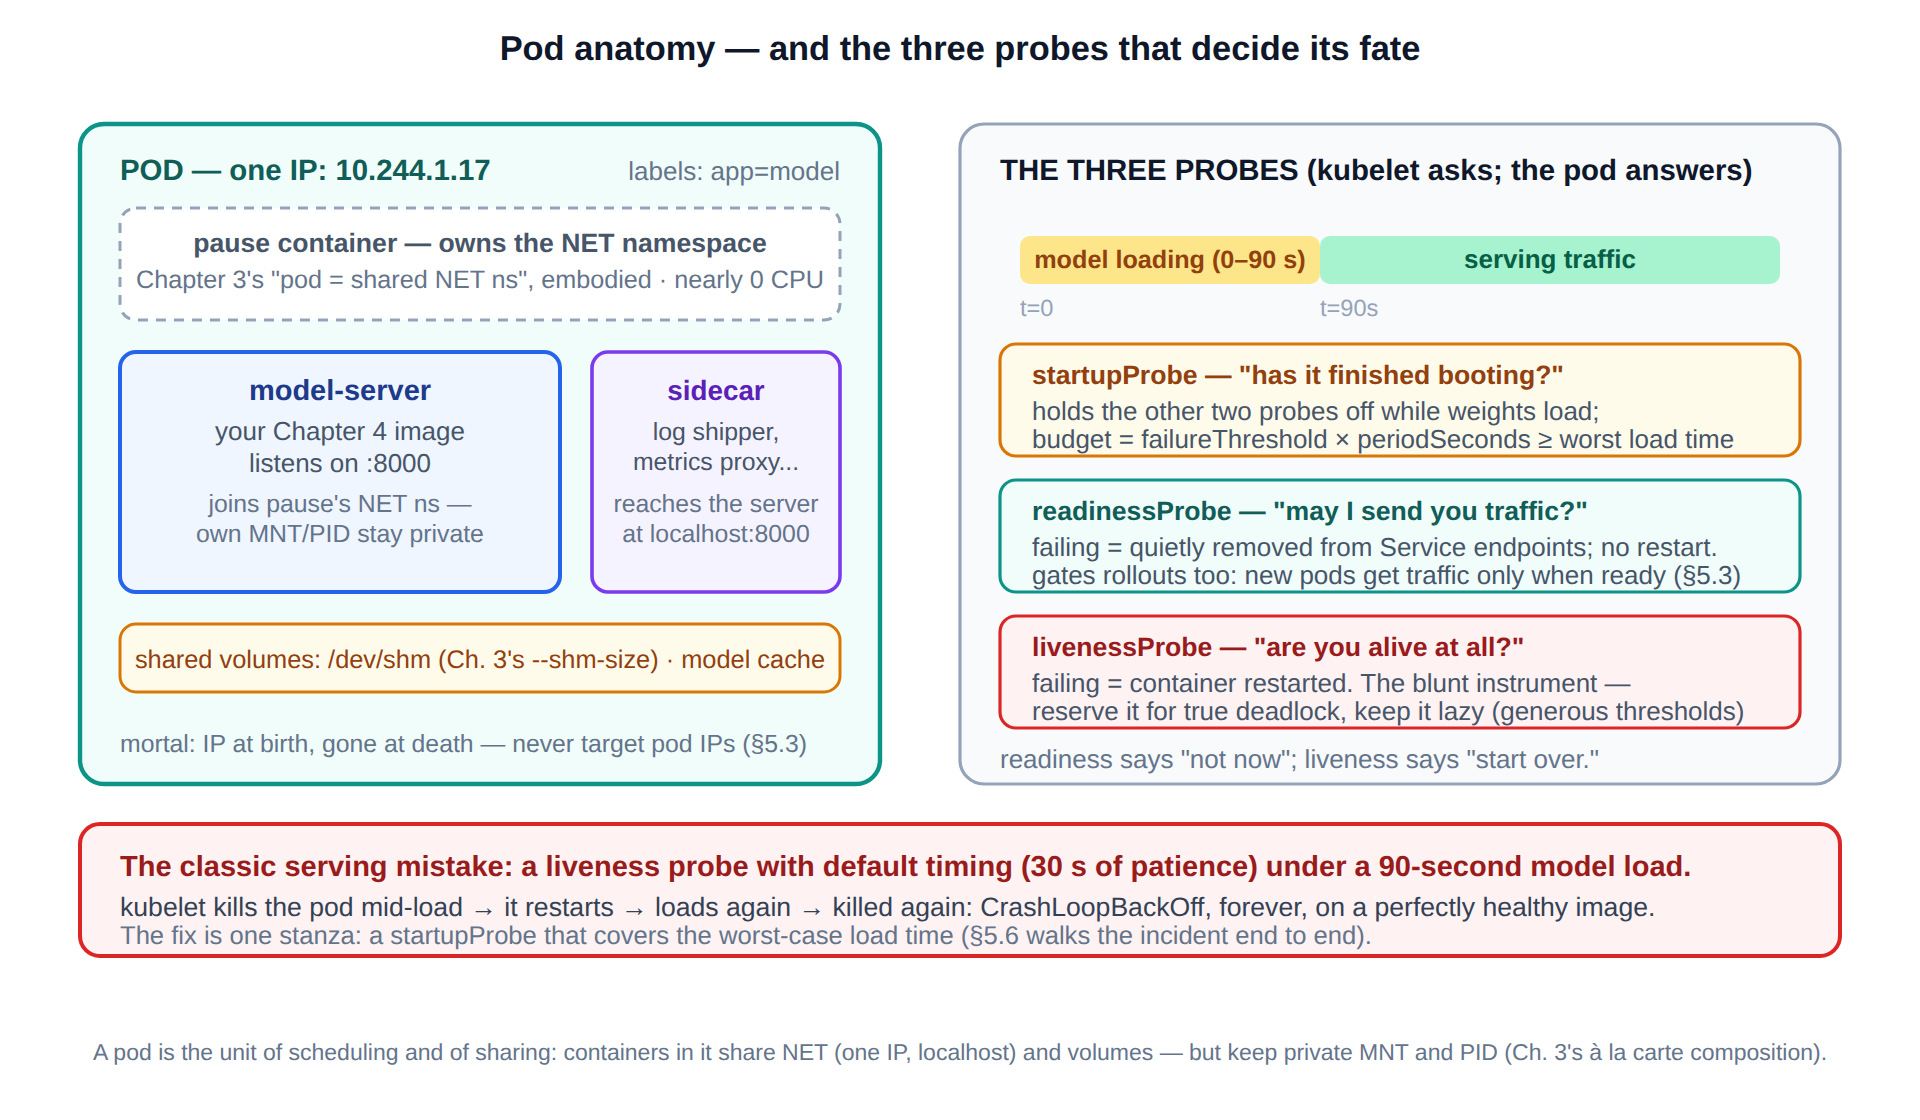
\includegraphics{figures/fig5-3_pod.png}}\\[3pt]
  \figcaption{Figure 5-3  Pod anatomy (left): pause owns the shared namespaces; containers join. The three probes (right): startup covers the model load, readiness gates traffic, liveness restarts the truly dead.}
\end{tbbfigure}

\subsection*{The manifest you will actually write}

Here is the full Deployment manifest for the course model server — worth reading line by line, because §5.4 and §5.6 each hang an entire section off one stanza of it:

\begin{terminalbox}
\begin{Verbatim}[breaklines=true,breakanywhere=true,fontsize=\small,formatcom=\color{tbbtermfg},codes=\tbbcodeactive]
apiVersion: apps/v1
kind: Deployment
metadata:
  name: model-server
spec:
  replicas: 3
  selector:
    matchLabels: { app: model }
  template:
    metadata:
      labels: { app: model }        # must match selector - membership tag
    spec:
      terminationGracePeriodSeconds: 30   # Ch. 3's SIGTERM tape, the knob
      containers:
      - name: server
        image: registry.example.com/team/model-server:v7
        ports: [ { containerPort: 8000 } ]
        resources:                  # sec. 5.4 lives here
          requests: { cpu: "1", memory: 1.2Gi }
          limits:   { cpu: "2", memory: 1.75Gi }
        startupProbe:               # covers the model load
          httpGet: { path: /healthz, port: 8000 }
          periodSeconds: 5
          failureThreshold: 36      # 36 x 5s = 3 min of grace
        readinessProbe:             # gates traffic
          httpGet: { path: /ready, port: 8000 }
          periodSeconds: 5
        livenessProbe:              # restarts the truly dead
          httpGet: { path: /healthz, port: 8000 }
          periodSeconds: 10
          failureThreshold: 3
\end{Verbatim}
\end{terminalbox}
\figcaption{Transcript 5-3  The course Deployment manifest. Three stanzas do the heavy lifting: labels (membership), resources (§5.4), probes (below and §5.6).}

\begin{terminalbox}
\begin{Verbatim}[breaklines=true,breakanywhere=true,fontsize=\small,formatcom=\color{tbbtermfg},codes=\tbbcodeactive]
$ kubectl apply -f model-server.yaml
deployment.apps/model-server created
$ kubectl get pods -o wide
NAME                            READY  STATUS    IP            NODE
model-server-7d4b9c6f5-8xk2p    1/1    Running   10.244.1.17   node-a
model-server-7d4b9c6f5-tq9wz    1/1    Running   10.244.2.31   node-b
model-server-7d4b9c6f5-fh5m8    0/1    Running   10.244.1.44   node-a
# 0/1 = running but not READY: the model is still loading.
# readiness is failing on purpose - and no traffic arrives yet.
\end{Verbatim}
\end{terminalbox}
\figcaption{Transcript 5-4  Applied and placed across nodes. Note the third pod: Running is about the process; READY is about willingness to serve. The gap between them is the model load.}

\subsection*{Probes: three questions, three different consequences}

The kubelet keeps asking every container three questions, and serving systems live or die by keeping the answers distinct. \textbf{startupProbe} — "have you finished booting?" — exists precisely for the slow starts that models cause: while it runs, the other two probes are suspended, and its budget (\code{failureThreshold × periodSeconds}; 3 minutes in Transcript 5-3) must cover the worst-case weight load. \textbf{readinessProbe} — "may I send you traffic?" — controls exactly one thing: membership in Service endpoints. Failing readiness does not restart anything; it quietly removes the pod from rotation, which is what you want while loading, during overload, or while draining. \textbf{livenessProbe} — "are you alive at all?" — is the blunt instrument: failure means the container is killed and restarted. It should test the process's own health (event loop responsive), never dependencies, and it should be \textit{lazy} — generous periods and thresholds.

Now the classic serving incident, in one sentence you can already parse: a liveness probe with default patience, pointed at a server whose model takes ninety seconds to load, kills the container mid-load, forever — \textbf{CrashLoopBackOff on a perfectly healthy image.} Section 5.6 stages the whole incident with transcripts, because you will meet it in the wild; the vaccine is the startupProbe stanza above, and the diagnostic habit is Transcript 5-4's distinction: Running is not Ready, and neither is dead.

\subsection*{Deployment: versioned fleets and bloodless rollouts}

A Deployment manages ReplicaSets, one per version of the pod template (the template's hash is right there in the pod names of Transcript 5-1). Change anything in the template — new image tag, new memory limit — and the Deployment creates a \textit{new} ReplicaSet and shifts pods between old and new at a governed pace: \code{maxSurge} (how many extras may exist during the shift) and \code{maxUnavailable} (how many may be missing). The serving-friendly setting is \code{maxSurge: 1, maxUnavailable: 0} — never dip below capacity; add one, wait for it to be \textbf{Ready}, retire one. And that "wait for Ready" is the load-bearing phrase: \textbf{readiness is what paces a rollout.} A new version that never becomes ready stalls the rollout at one surge pod — old version still serving, blast radius one pod — which is the system quietly saving you from yourself.

\begin{terminalbox}
\begin{Verbatim}[breaklines=true,breakanywhere=true,fontsize=\small,formatcom=\color{tbbtermfg},codes=\tbbcodeactive]
$ kubectl set image deployment/model-server server=.../model-server:v8
deployment.apps/model-server image updated
$ kubectl rollout status deployment/model-server
Waiting for rollout: 1 out of 3 new replicas are available...
$ kubectl get pods
NAME                            READY   STATUS        RESTARTS   AGE
model-server-7d4b9c6f5-8xk2p    1/1     Running       0          2d
model-server-7d4b9c6f5-tq9wz    1/1     Terminating   0          2d
model-server-6f8d5b9c44-2mwpx   1/1     Running       0          38s
model-server-6f8d5b9c44-9qk7d   0/1     Running       0          6s
# surge pod loading; an old pod drains only after a new one is Ready.
# regret it? one command points back at the old ReplicaSet:
$ kubectl rollout undo deployment/model-server
\end{Verbatim}
\end{terminalbox}
\figcaption{Transcript 5-5  A rolling update, mid-flight: v8 pods joining as they become Ready, v7 pods terminating only then. Rollback is repointing at the previous ReplicaSet, which was kept at scale 0.}

Look at that \code{Terminating} pod with Chapter 3 eyes: the kubelet sends \textbf{SIGTERM to PID 1}, waits \code{terminationGracePeriodSeconds} (the manifest set 30), then SIGKILLs. Everything §3.2 taught — the exec-form CMD, the handler that stops accepting and drains, tini if you need it — is what makes that \code{Terminating} second invisible to clients. Kubernetes did not solve graceful shutdown; it \textit{schedules} it. Your handler still does the work, at every single rollout, node drain, and scale-down for the rest of this course.

\subsection*{Service: one stable name in front of mortal pods}

Pods are cattle: they get an IP at birth and lose it at death, and Transcript 5-5 just showed you how routine death is. No client can be asked to chase that. A \textbf{Service} is the fix: a stable virtual IP and DNS name (\code{model-svc.ml.svc.cluster.local}, courtesy of CoreDNS) in front of whichever pods currently match a \textbf{label selector} \textit{and} pass readiness. The matching pods' IPs form the \textbf{endpoints} list, updated live by a controller; \textbf{kube-proxy} programs the node's packet path (iptables or IPVS) so that connections to the virtual IP are DNAT-rewritten to one healthy backend. You met this exact mechanism in Chapter 3's \code{-p 8080:8000} packet walk — a published port was one NAT rule; a Service is the same trick, cluster-wide and health-aware (Figure 5-4). In MSA terms, this is \textbf{service discovery, solved by the platform}: consumers know a name, never a topology.

\begin{tbbfigure}
  \adjustbox{max width=0.94\linewidth,max totalheight=0.46\textheight}{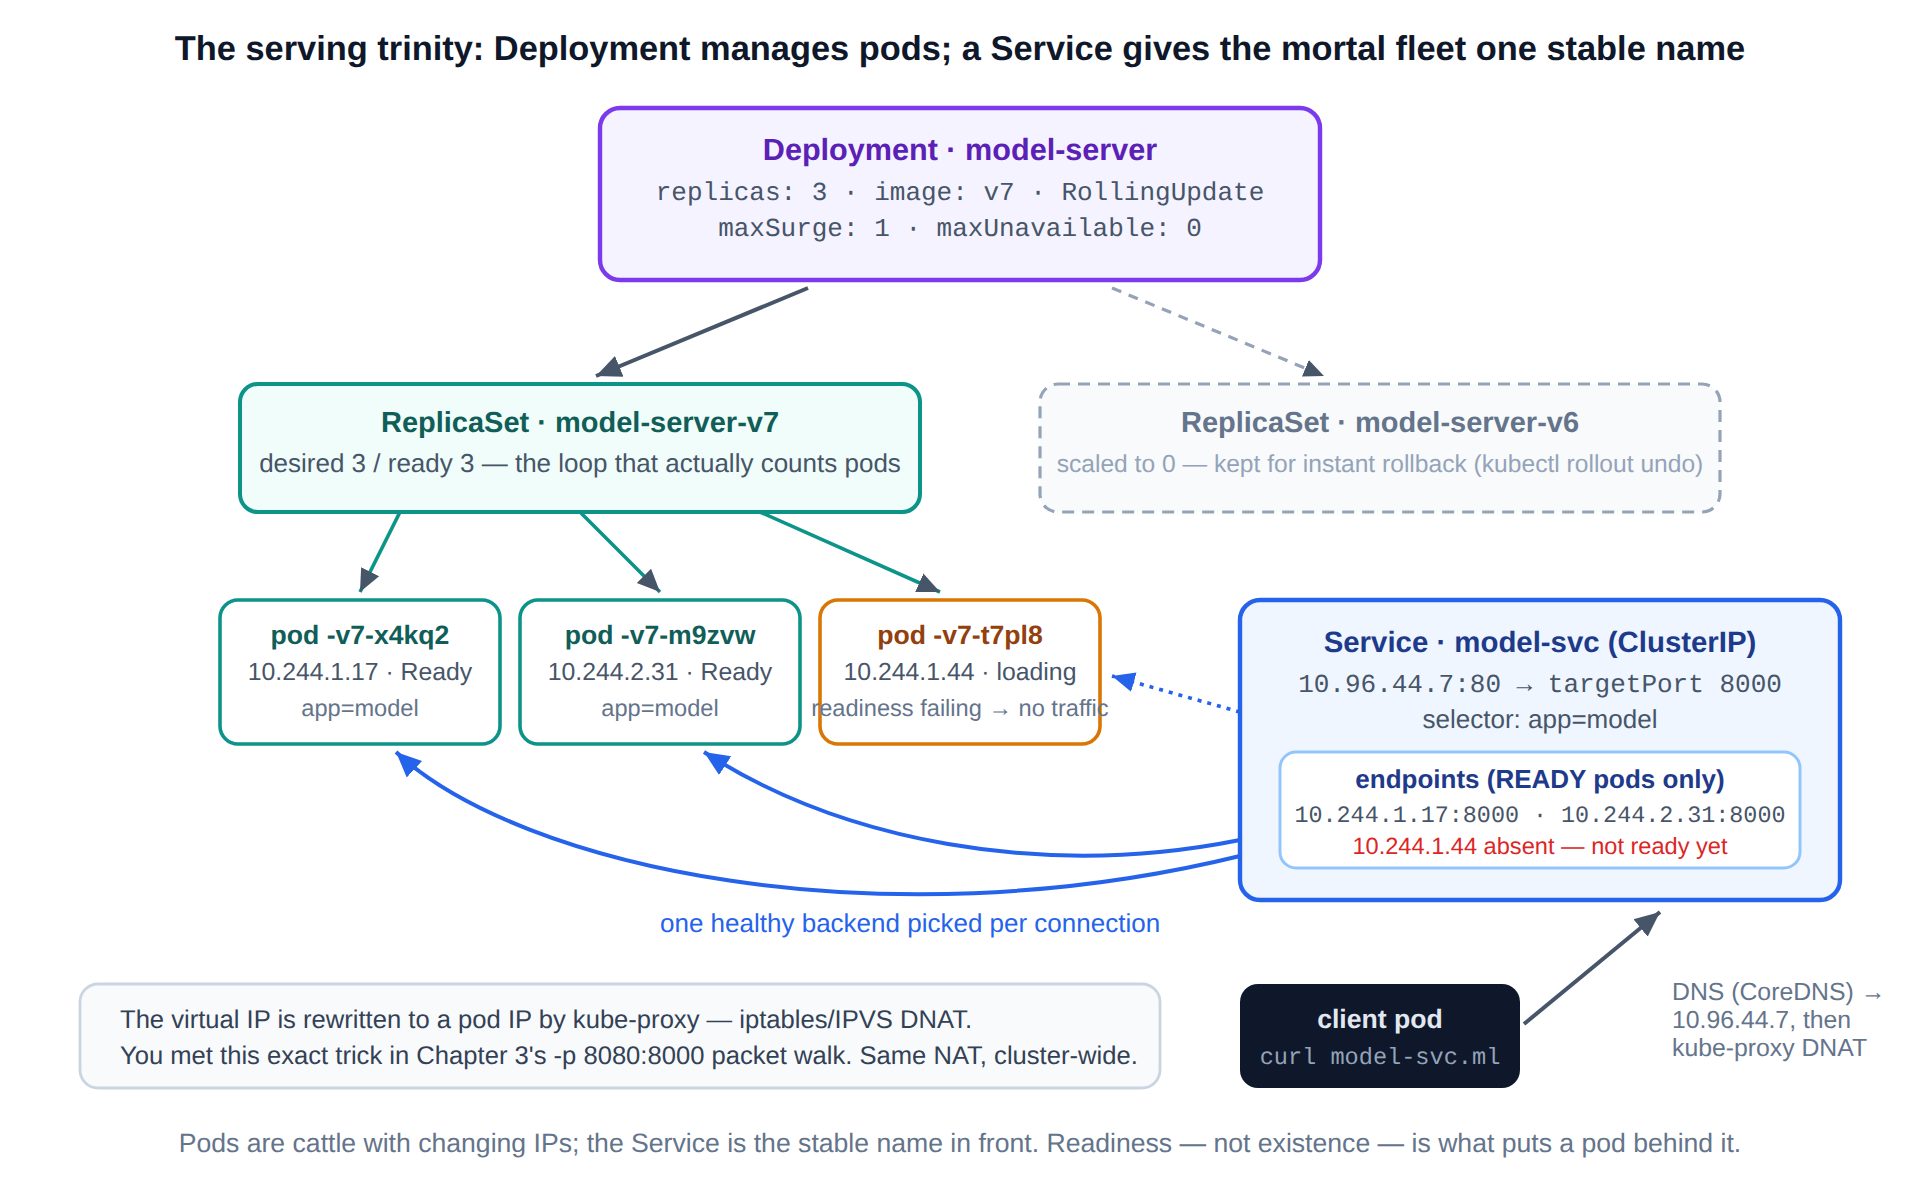
\includegraphics{figures/fig5-4_deploy_svc.png}}\\[3pt]
  \figcaption{Figure 5-4  Deployment → ReplicaSet → pods, with a Service in front. The endpoints list contains READY pods only — which is how loading pods and draining pods drop out of traffic automatically.}
\end{tbbfigure}

\begin{terminalbox}
\begin{Verbatim}[breaklines=true,breakanywhere=true,fontsize=\small,formatcom=\color{tbbtermfg},codes=\tbbcodeactive]
$ kubectl expose deployment model-server --name=model-svc \
    --port 80 --target-port 8000
service/model-svc exposed
$ kubectl get svc model-svc
NAME        TYPE        CLUSTER-IP     EXTERNAL-IP   PORT(S)   AGE
model-svc   ClusterIP   10.96.44.7     <none>        80/TCP    5s
$ kubectl get endpoints model-svc
NAME        ENDPOINTS                             AGE
model-svc   10.244.1.17:8000,10.244.2.31:8000     5s
# two backends - the third pod is still loading (not Ready).
# from any pod in the cluster:
$ curl -s http://model-svc.default/predict -d '{"x": [1,2]}'
{"y": 0.87, "model": "v7"}
\end{Verbatim}
\end{terminalbox}
\figcaption{Transcript 5-6  A Service in front of the fleet: virtual IP, DNS name, and an endpoints list that only ever contains pods answering their readiness probe.}

Three Service types form a ladder of exposure. \textbf{ClusterIP} (the default above) is reachable only inside the cluster — right for model servers that sit behind other services. \textbf{NodePort} opens a high port (30000–32767) on every node — the minikube lab's way out. \textbf{LoadBalancer} asks the cloud for a real external load balancer wired to those node ports — the managed-cluster way, and the piece Week 6 extends with API gateways, TLS, and auth in front. One name to file now: a Service load-balances \textit{connections}, not requests — long-lived connections (streaming, gRPC multiplexing) can defeat it, a wrinkle that returns with LLM streaming in Week 11.

One more habit while the trinity is fresh: \textbf{namespaces}. They scope names, quotas, and access — the lab creates everything inside a namespace called \code{ml} rather than \code{default}, because every real cluster you touch will be divided this way (and Week 13's CI/CD pipelines will deploy to per-environment namespaces).

\begin{calloutbox}{tbbpurple}{tbbpurplefill}
{\normalsize\bfseries\color{tbbpurple}Think About It}\par\vspace{3pt}
\begin{tbbitemize}
  \item Two Deployments — model-server-v7 and an experimental v8 — accidentally both carry the label app=model, and one Service selects app=model. Describe exactly what clients experience, why no component flags an error, and where you would first see it. (This misconfiguration, done on purpose, is called a canary — Week 13.)
  \item Rolling updates wait for readiness, not merely for the container to start. Construct the concrete disaster that maxSurge: 1, maxUnavailable: 0 with only container-started gating would cause for a 90-second-loading model under full traffic.
  \item A pod can be alive (liveness passing), never ready (readiness failing), and never restarted — indefinitely. Argue that this non-terminating state is a feature, then name the §5.6 failure it becomes when unintended.
\end{tbbitemize}
\end{calloutbox}

\section{requests, limits, and QoS: Chapter 3 at Fleet Scale}

The \code{resources:} stanza in Transcript 5-3 is eight lines long and carries more operational weight than the rest of the manifest combined. Its central subtlety is that the stanza is read by \textbf{two different machines with two different jobs} (Figure 5-5). \textbf{requests} are read by the \textit{scheduler}, at placement time, as arithmetic: a pod fits on a node if the node's \textbf{allocatable} capacity minus the sum of already-placed requests still covers this pod's requests. That is all requests are — planning numbers. \textbf{They are never enforced at runtime.} A pod requesting 1 CPU may happily use 3 if the node has slack. \textbf{limits}, by contrast, are read by the \textit{kubelet} and become — via Chapter 4's runtime stack — exactly the cgroup files of Chapter 3, enforced by the kernel every millisecond.

\begin{tbbfigure}
  \adjustbox{max width=0.94\linewidth,max totalheight=0.46\textheight}{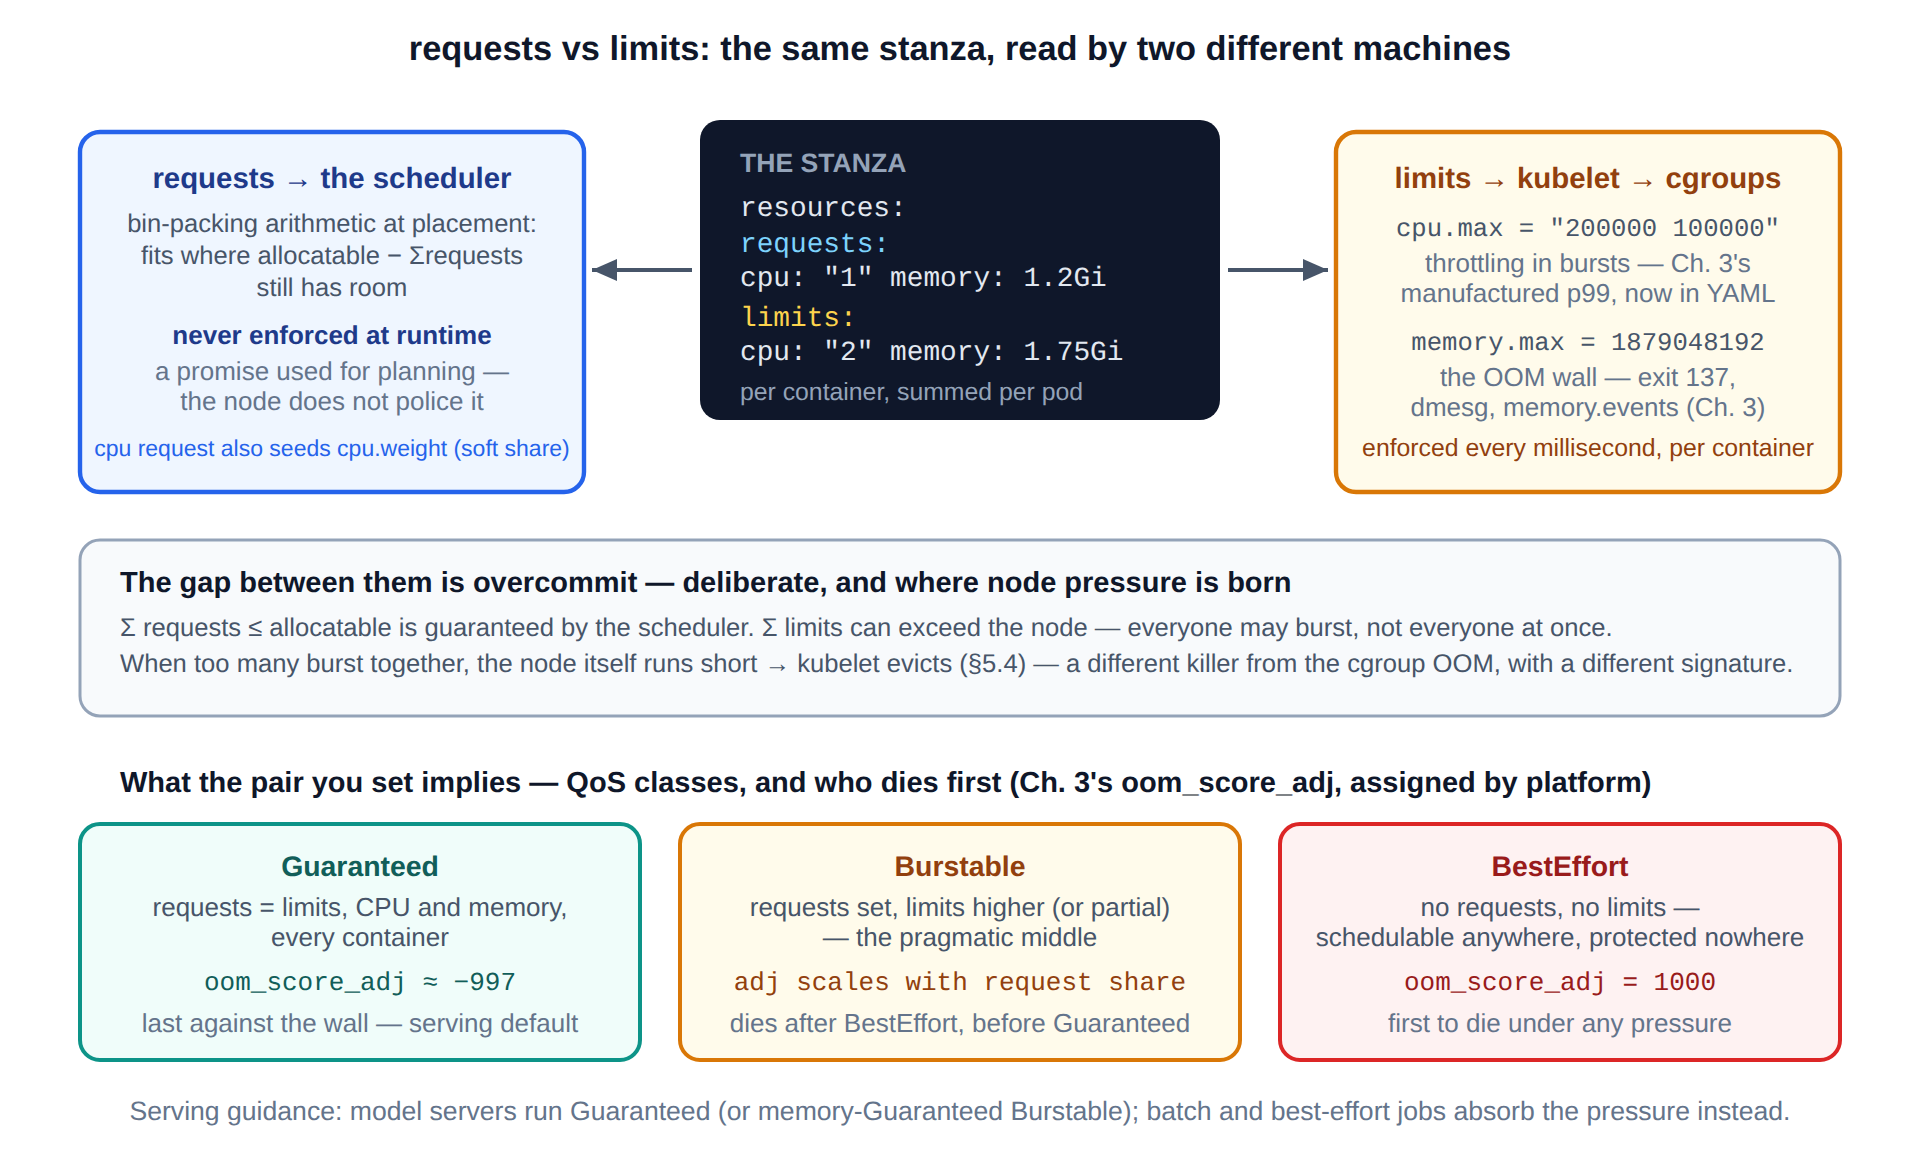
\includegraphics{figures/fig5-5_requests_limits.png}}\\[3pt]
  \figcaption{Figure 5-5  One stanza, two readers: requests feed the scheduler's bin-packing; limits become cpu.max and memory.max. The gap between them is deliberate overcommit — and the birthplace of node pressure.}
\end{tbbfigure}

\subsection*{The thesis transcript: YAML in, cgroup files out}

Chapter 3 opened by interrogating a Docker container from the host and finding a process with cgroup files attached. Run the same interrogation on Kubernetes and the chapter's thesis closes:

\begin{terminalbox}
\begin{Verbatim}[breaklines=true,breakanywhere=true,fontsize=\small,formatcom=\color{tbbtermfg},codes=\tbbcodeactive]
$ kubectl get pod model-server-7d4b9c6f5-8xk2p \
    -o jsonpath='{.spec.nodeName} {.status.qosClass}'
node-a Burstable
$ minikube ssh                        # onto the node itself
node-a $ ps aux | grep uvicorn        # the server is just a process (Ch. 3)
root  41320  2.1  7.8  ...  uvicorn serve:app --port 8000
node-a $ cat /proc/41320/cgroup
0::/kubepods.slice/kubepods-burstable.slice/kubepods-...-pod9f31.slice/...
node-a $ cd /sys/fs/cgroup/kubepods.slice/kubepods-burstable.slice/...
node-a $ cat memory.max
1879048192                            # = 1.75Gi, your YAML, in bytes
node-a $ cat cpu.max
200000 100000                         # = limits.cpu "2", Ch. 3 grammar
node-a $ cat cpu.weight
39                                    # from requests.cpu "1" - soft share
\end{Verbatim}
\end{terminalbox}
\figcaption{Transcript 5-7  The chain closed by hand: YAML limits have become memory.max and cpu.max on the node; the CPU request became cpu.weight. Kubernetes is Chapter 3 with a database in front.}

Read the three files against Chapter 3 and every behavior follows. \code{memory.max = 1879048192} means the pod meets \textbf{the same OOM killer, with the same exit 137, the same dmesg confession, the same sizing playbook} — §3.6 applies verbatim, and \code{kubectl describe} will echo it as \code{Last State: OOMKilled}. \code{cpu.max = "200000 100000"} means the pod can be \textbf{throttled in bursts} — §3.3's manufactured p99, now set by a YAML line. And \code{cpu.weight} (derived from requests) is the polite, work-conserving share that only matters under contention. The table you should carry:

\begin{tbbtablewrap}
  \begin{tabular}{@{}>{\raggedright\arraybackslash}m{\dimexpr 0.3085\tbltextwidth-2\tabcolsep\relax} >{\raggedright\arraybackslash}m{\dimexpr 0.3511\tbltextwidth-2\tabcolsep\relax} >{\raggedright\arraybackslash}m{\dimexpr 0.3404\tbltextwidth-2\tabcolsep\relax}@{}}
  \arrayrulecolor{tbbnavy}\specialrule{1pt}{0pt}{0pt}
  \rowcolor{tbbtablehead}{\centering \bfseries\color{tbbnavy}You write (YAML)} & {\centering \bfseries\color{tbbnavy}It becomes} & {\centering \bfseries\color{tbbnavy}Character} \\
  \arrayrulecolor{tbbnavy}\specialrule{0.7pt}{0pt}{2pt}
  {requests.cpu: "1"} & {scheduler arithmetic + cpu.weight} & {planning + soft share; work-conserving} \\
  \arrayrulecolor{tbbtableborder}\hline
  {requests.memory: 1.2Gi} & {scheduler arithmetic (+ eviction rank)} & {planning only — no kernel object} \\
  \arrayrulecolor{tbbtableborder}\hline
  {limits.cpu: "2"} & {\textcolor{tbbamberdark}{cpu.max = "200000 100000"}} & {hard quota; throttles in bursts (§3.3)} \\
  \arrayrulecolor{tbbtableborder}\hline
  {limits.memory: 1.75Gi} & {\textcolor{tbbred}{memory.max = 1879048192}} & {hard wall; OOM killer (§3.6)} \\
  \arrayrulecolor{tbbtableborder}\hline
  {nvidia.com/gpu: 1} & {device-plugin allocation (§5.5)} & {integer; no cgroup — no kernel referee} \\
  \arrayrulecolor{tbbnavy}\specialrule{1pt}{2pt}{0pt}
  \end{tabular}\par
  \figcaption{Table 5-1  The translation, line by line}
\end{tbbtablewrap}

\subsection*{CPU: request generously, limit reluctantly}

For CPU, the two knobs inherit Chapter 3's two personalities, and the serving guidance falls out mechanically. The request is a \textit{reservation} — it decides placement and, through \code{cpu.weight}, guarantees a proportional floor under contention while wasting nothing when neighbors idle. The limit is a \textit{ceiling} — \code{cpu.max} — and §3.3's arithmetic showed what ceilings do to tail latency: a request needing 30 ms of CPU under a 0.2-CPU quota takes 110–190 ms, with the profiler blind. So: \textbf{set CPU requests honestly} (they are your p99 insurance under noisy neighbors), and \textbf{be reluctant with CPU limits} on latency-critical pods — an idle core spent absorbing a burst is cheaper than a throttled window at p99. Two honest complications: platform teams often \textit{require} limits (billing hygiene, runaway protection), and Guaranteed QoS — next paragraphs — requires requests = limits. Teams that need both pinned performance and QoS use generous equal values, or the kubelet's static CPU-manager policy, which grants Guaranteed integer-CPU pods \textit{exclusive cores} — Chapter 2's dedicated-core idea, reappearing at the kubelet.

\subsection*{Memory: the gap, the pressure, and the second killer}

Memory is where the requests/limits gap earns its own vocabulary. The scheduler guarantees Σrequests ≤ allocatable per node; it says nothing about limits, so \textbf{Σlimits routinely exceeds the node} — that is overcommit, and it is a feature: everyone may burst, on the bet that not everyone bursts at once. When the bet loses — several replicas spike together, per §3.6 inference memory is \textit{spiky by nature} — the \textbf{node itself} runs short before any single pod hits its own wall. The kernel's node-level OOM killer would be chaos; Kubernetes prefers order: the \textbf{kubelet evicts} — it picks victims by QoS class and usage-over-request, kills them cleanly, and marks them \code{Evicted}. You now know two distinct killers, and telling them apart is a §5.6 skill:

\begin{tbbtablewrap}
  \begin{tabular}{@{}>{\raggedright\arraybackslash}m{\dimexpr 0.2340\tbltextwidth-2\tabcolsep\relax} >{\raggedright\arraybackslash}m{\dimexpr 0.3830\tbltextwidth-2\tabcolsep\relax} >{\raggedright\arraybackslash}m{\dimexpr 0.3830\tbltextwidth-2\tabcolsep\relax}@{}}
  \arrayrulecolor{tbbnavy}\specialrule{1pt}{0pt}{0pt}
  \rowcolor{tbbtablehead}{\centering \bfseries\color{tbbnavy}} & {\centering \bfseries\color{tbbnavy}cgroup OOM kill (Ch. 3)} & {\centering \bfseries\color{tbbnavy}node-pressure eviction} \\
  \arrayrulecolor{tbbnavy}\specialrule{0.7pt}{0pt}{2pt}
  {\textbf{trigger}} & {this pod crossed its own memory.max} & {the node ran short (overcommit bet lost)} \\
  \arrayrulecolor{tbbtableborder}\hline
  {\textbf{executioner}} & {kernel OOM killer — SIGKILL} & {kubelet — graceful pod termination} \\
  \arrayrulecolor{tbbtableborder}\hline
  {\textbf{blast radius}} & {one container} & {chosen victims, QoS-ordered, node-wide} \\
  \arrayrulecolor{tbbtableborder}\hline
  {\textbf{signature}} & {\textcolor{tbbred}{OOMKilled · exit 137 · dmesg}} & {\textcolor{tbbpurple}{status Evicted · "node was low on memory"}} \\
  \arrayrulecolor{tbbtableborder}\hline
  {\textbf{first fix}} & {resize to peak or bound batch (§3.6)} & {honest requests; Guaranteed QoS for serving} \\
  \arrayrulecolor{tbbnavy}\specialrule{1pt}{2pt}{0pt}
  \end{tabular}\par
  \figcaption{Table 5-2  Two killers, two signatures}
\end{tbbtablewrap}

\subsection*{QoS classes: who dies first is a setting}

The kubelet's eviction order — and the node OOM killer's scoring, should it ever come to that — is not guesswork; it is Chapter 3's \code{oom\_score\_adj}, assigned by platform according to your requests/limits pattern. \textbf{Guaranteed} (requests = limits for both CPU and memory, every container) earns ≈ −997: nearly untouchable. \textbf{BestEffort} (nothing set) earns +1000: first against the wall, always. \textbf{Burstable} (everything in between) scales with how far usage exceeds requests. The serving translation writes itself: \textbf{model servers should run Guaranteed} — at minimum, memory requests = limits — so that when an overcommitted node feels pressure, it is the batch jobs and best-effort experiments that die, not the pod holding p99. (Kubernetes adds a second, orthogonal knob — PriorityClass — which orders \textit{preemption and eviction between workloads}; QoS orders \textit{kill priority on a node}. Week 12's autoscaling story uses both.)

\begin{calloutbox}{tbbblue}{tbbbluefill}
{\normalsize\bfseries\color{tbbblue}Worked example — packing a node, by hand}\par\vspace{3pt}
Take a general-purpose 8-vCPU / 32 GiB node. After system and kubelet reservations, \textbf{allocatable ≈ 7.5 vCPU and 29 GiB} (Transcript 5-8 shows where to read this). Per-node daemons (log shipper, monitoring agent, kube-proxy) request ≈ 0.3 vCPU and 0.5 GiB. The course model server requests \code{cpu: 1, memory: 1.2Gi} (limits 2 / 1.75Gi).

\begin{tbbitemize}
  \item \textbf{CPU math:} (7.5 − 0.3) / 1 = \textbf{7 replicas} fit by CPU requests.
  \item \textbf{Memory math:} (29 − 0.5) / 1.2 ≈ \textbf{23 replicas} fit by memory requests.
\end{tbbitemize}

The node is \textbf{CPU-bound for this workload}: 7 replicas per node, with memory to spare — so paying for a memory-heavy instance type would be waste (Chapter 1's cost lens; instance choice should follow the binding dimension). Now check the overcommit exposure: 7 replicas × limits = 14 vCPU and 12.25 GiB. CPU limits (14) exceed allocatable (7.5) — legal, and it means simultaneous bursts are settled by cpu.weight in proportion to requests; p99 depends on honest requests. Memory limits (12.25 GiB) sit far below 29 GiB — this packing cannot even in principle trigger node memory pressure, a deliberately conservative posture for a serving node.

Re-run the same arithmetic for a 7B-parameter INT8 LLM server requesting \code{cpu: 2, memory: 9Gi}: memory now binds — (29 − 0.5) / 9 = \textbf{3 replicas} — and the right node family flips from compute-optimized to memory-optimized. Two minutes of division decides the instance family; Week 12's FinOps section builds the full cost model on exactly this habit.
\end{calloutbox}

\vspace{3.0pt}

\begin{calloutbox}{tbbpurple}{tbbpurplefill}
{\normalsize\bfseries\color{tbbpurple}Think About It}\par\vspace{3pt}
\begin{tbbitemize}
  \item A pod sets requests (1 CPU / 1 Gi) but no limits. Name its QoS class, what happens when it leaks memory on an otherwise-idle node, and who is endangered first when a \textit{neighbor} leaks instead.
  \item Why does the scheduler ignore limits entirely? Construct the argument from overcommit-as-a-feature, then name one workload mix where scheduling on limits would clearly be better.
  \item All 7 replicas from the worked example show nr\_throttled climbing at peak traffic (limits.cpu 2 × 7 = 14 on 7.5 allocatable). Using §3.3 and this section, explain the p99 symptom and propose two distinct remedies with their costs.
\end{tbbitemize}
\end{calloutbox}

\section{GPUs and the Scheduler}

Everything so far treated nodes as interchangeable. The moment GPUs enter, placement becomes the expensive decision: the spread between a well-placed and badly-placed GPU fleet is thousands of dollars a month, and — unlike CPU — a mistake cannot be absorbed by overcommit, because \textbf{GPUs do not overcommit}. This section is the scheduler section, with GPUs as the motivating hard case.

\subsection*{Filter, score, bind — the pass itself}

For each unbound pod, the scheduler runs a two-phase pass (Figure 5-6). \textbf{Filtering} removes every node that \textit{cannot} run the pod — insufficient allocatable resources against requests, missing extended resources, node selectors or affinity unmet, taints not tolerated. What survives is the feasible set; if it is empty, the pod stays \textbf{Pending}, and — worth italics — \textit{the event message enumerates exactly which filters failed and how many nodes failed each} (§5.6 reads one). \textbf{Scoring} then ranks the feasible set with soft preferences — spread across zones, prefer less-loaded (or more-loaded; below), image already present — and \textbf{bind} writes the winner's name into the pod object. The scheduler's output is one field on one object; everything after is §5.2's chain.

\begin{tbbfigure}
  \adjustbox{max width=0.94\linewidth,max totalheight=0.46\textheight}{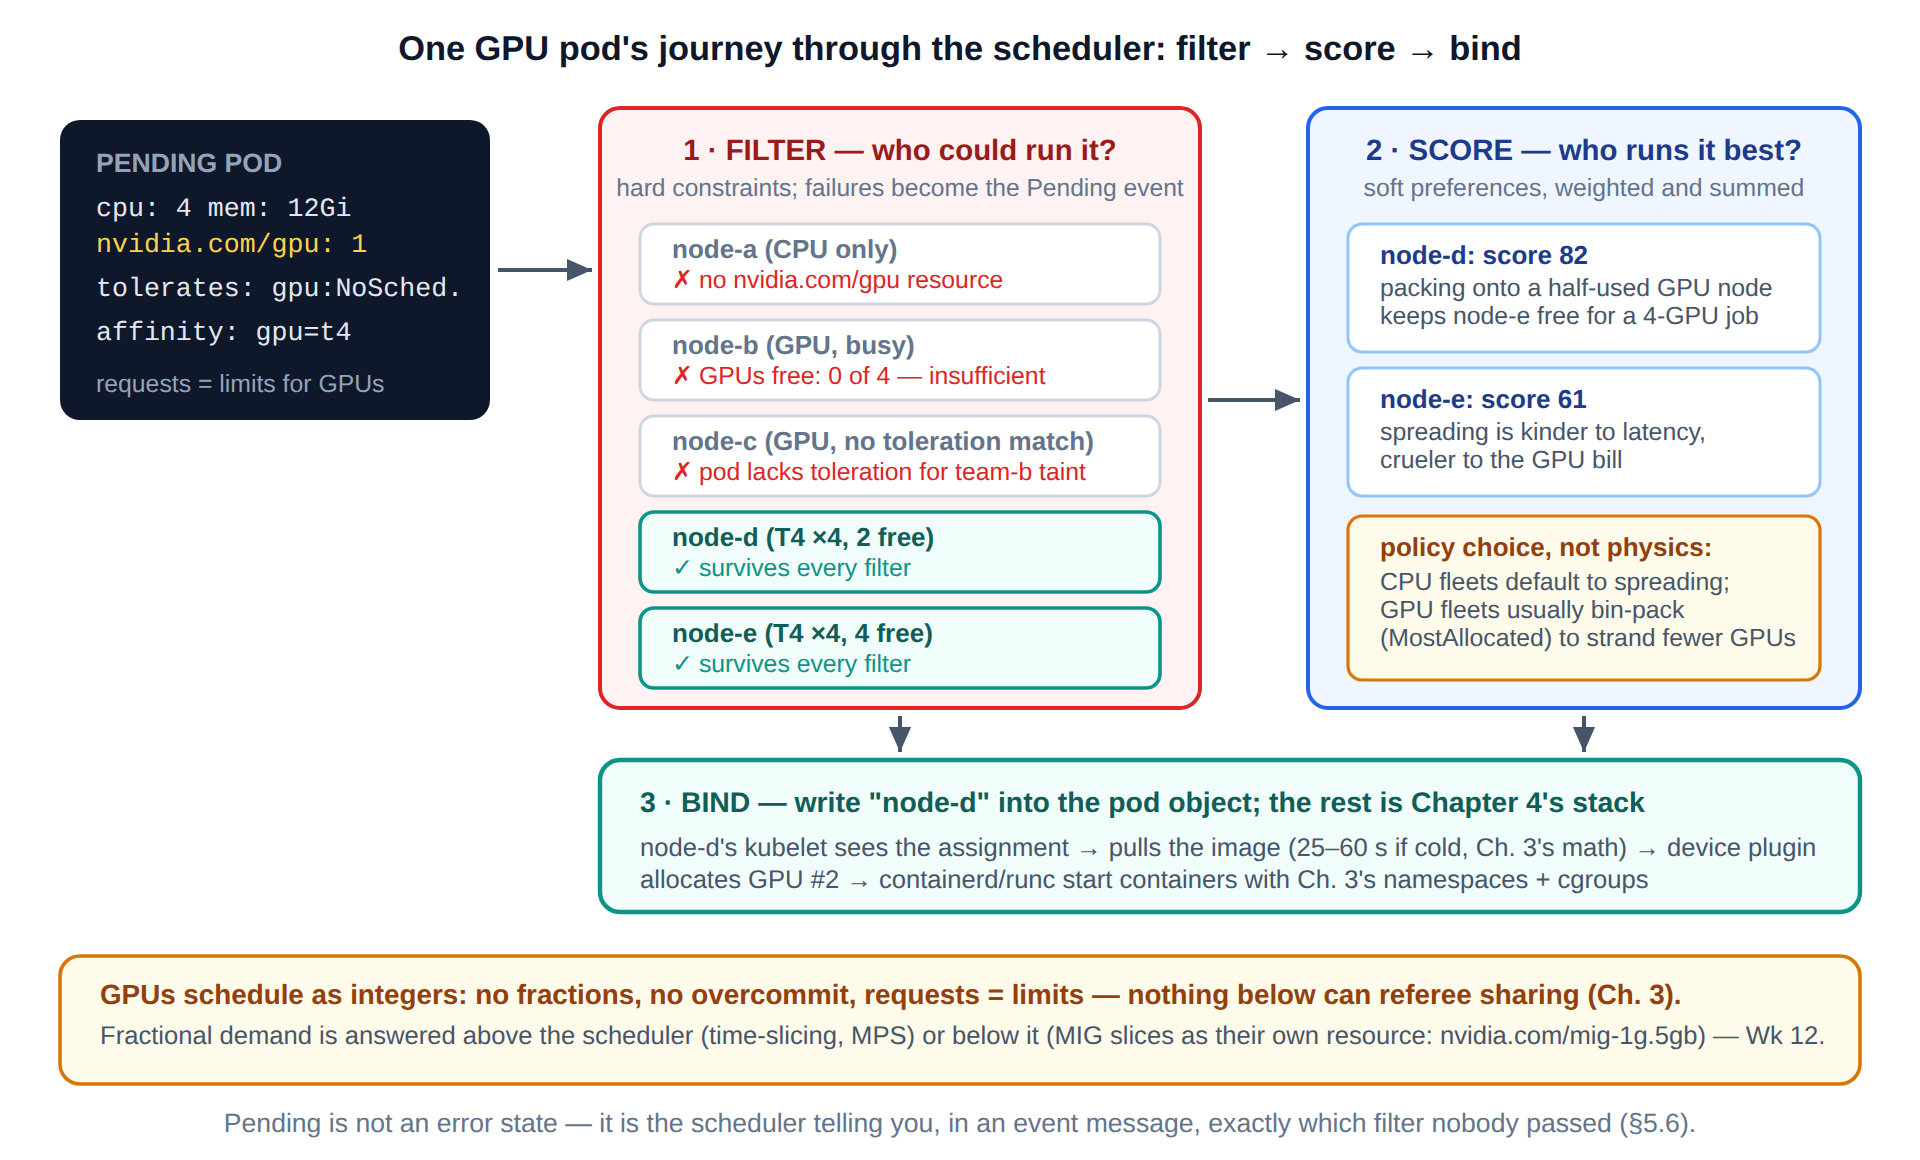
\includegraphics{figures/fig5-6_scheduler.png}}\\[3pt]
  \figcaption{Figure 5-6  A GPU pod's scheduling pass: filters eliminate (and their failures become the Pending event); scores rank; bind writes a name. Packing versus spreading is a policy choice with a GPU-sized price tag.}
\end{tbbfigure}

\subsection*{GPUs are extended resources: integers, no overcommit, requests = limits}

A GPU enters Kubernetes as an \textbf{extended resource}: Chapter 4's device plugin, running on each GPU node, advertises \code{nvidia.com/\allowbreak gpu: 4} to the kubelet, which reports it in the node's capacity. Pods consume it with one stanza — and three rules that are stricter than anything CPU or memory imposed: the quantity must be an \textbf{integer}; \textbf{requests must equal limits}; and there is \textbf{no overcommit, ever}. When the pod starts, the device plugin allocates \textit{specific} GPUs (by index/UUID) and injects them into the container — Chapter 4's \code{/\allowbreak dev/\allowbreak nvidia*} plumbing.

\begin{terminalbox}
\begin{Verbatim}[breaklines=true,breakanywhere=true,fontsize=\small,formatcom=\color{tbbtermfg},codes=\tbbcodeactive]
# in the pod spec - the entire GPU ask:
        resources:
          limits:
            nvidia.com/gpu: 1        # integer; requests implied equal

$ kubectl describe node gpu-node-3 | sed -n '/Capacity/,/pods/p'
Capacity:
  cpu:                48
  memory:             196Gi
  nvidia.com/gpu:     4
Allocatable:
  cpu:                47
  memory:             186Gi
  nvidia.com/gpu:     4
$ kubectl describe node gpu-node-3 | grep -A4 "Allocated resources"
Allocated resources:
  Resource           Requests      Limits
  cpu                18 (38%)      36 (76%)
  memory             88Gi (47%)    120Gi (64%)
  nvidia.com/gpu     2             2          # 2 of 4 in use
\end{Verbatim}
\end{terminalbox}
\figcaption{Transcript 5-8  A GPU node as the scheduler sees it: the device plugin's advertisement in Capacity/Allocatable, and current GPU occupancy. Note CPU overcommitted in limits; GPUs never.}

Why the strictness? Chapter 3 already handed you the answer: \textbf{cgroups have no GPU controller.} For CPU, overcommit is safe because cpu.weight arbitrates contention work-conservingly; for memory, memory.max plus the OOM killer enforce the wall. For a GPU there is no kernel mechanism to referee two containers' compute or partition VRAM — so Kubernetes refuses to promise what nothing below it can enforce. One GPU, one owner. Fractional GPU \textit{demand} is real (a small INT8 model rarely fills an A100), but the answer lives outside this section's scheduler: \textbf{time-slicing} (the device plugin advertises N virtual copies per GPU — placement without isolation: neighbors share VRAM unprotected), \textbf{MPS} (spatial sharing, still cooperative), or \textbf{MIG} (Chapter 2's hardware partitions, each advertised as its own extended resource such as \code{nvidia.com/\allowbreak mig-1g.5gb} — real isolation, schedulable like any resource). Week 12 turns this menu into configuration; this chapter's job is that you know \textit{why} the menu exists.

\subsection*{Placement controls: taints push, affinity pulls}

Two mechanisms steer pods relative to special nodes, and GPU fleets need both directions. A \textbf{taint} on a node repels pods that do not explicitly tolerate it — managed GPU node pools ship tainted (\code{nvidia.com/\allowbreak gpu=present:NoSchedule}) precisely so that a stray log-processing Deployment never occupies a \$3-per-hour node just because it had free CPU. A \textbf{toleration} merely unlocks the door; it does not aim the pod. Aiming is \textbf{nodeSelector / node affinity} against labels: \code{gpu=t4} versus \code{gpu=a100} matters because Chapter 2's fleet table is real — a model validated on T4 economics may be waste on an A100, and Week 10's quantized models change the right answer per model. The GPU pod therefore carries both: a toleration (permission) and an affinity (intent).

\subsection*{Packing versus spreading: scheduling policy is a line item}

For stateless CPU fleets, the default scoring instinct — spread pods out, keep nodes evenly loaded — is healthy: it smooths noisy neighbors and survives node loss gracefully. For GPU fleets it is quietly expensive, in two ways. First, \textbf{fragmentation}: spreading 1-GPU pods across nodes leaves every node partially used, so a later multi-GPU pod finds no single node with enough free GPUs — Pending with plenty of total capacity free. Second, \textbf{stranding}: a GPU node whose CPUs or memory are consumed by non-GPU pods has GPUs that are free, priced, and unusable. The remedies are policy, not code: score GPU nodes for \textbf{bin-packing} (the scheduler's MostAllocated strategy) so used nodes fill and empty nodes stay empty — which also hands Week 12's cluster autoscaler whole idle nodes it can delete; taint GPU nodes so nothing CPU-shaped lands there; and keep GPU pods' CPU requests honest so a node's CPUs are not exhausted at two of four GPUs used.

\begin{calloutbox}{tbbamber}{tbbamberfill}
{\normalsize\bfseries\color{tbbamberdark}Worked example — what fragmentation costs}\par\vspace{3pt}
A cluster has 4 nodes × 4 A100s (on-demand ≈ \textbf{\$3/GPU-hour} — representative). Sixteen 1-GPU serving pods arrive; a spread-scoring scheduler places 4 per node — tidy, fully used, no waste \textit{yet}. Traffic falls at night; the fleet scales to 6 pods. Spread keeps \textasciitilde{}1–2 pods per node: \textbf{four nodes running, 10 idle GPUs still billed} ≈ 10 × \$3 × 24 ≈ \textbf{\$720/day of idle}, and the autoscaler can delete nothing (every node is occupied).

Same cluster, bin-packing: 6 pods fill 1.5 nodes → two nodes run, two drain empty and are deleted; idle spend collapses to ≈ \$144/day. And when a 4-GPU training job arrives at dawn, packed placement has a whole free node to give it; spread placement reports \textbf{Pending — 0/4 nodes have 4 free GPUs} while 10 GPUs sit free in fragments. Fragmentation is Pending with money attached.
\end{calloutbox}

\vspace{3.0pt}

\begin{calloutbox}{tbbpurple}{tbbpurplefill}
{\normalsize\bfseries\color{tbbpurple}Think About It}\par\vspace{3pt}
\begin{tbbitemize}
  \item State precisely why GPU requests must equal limits while CPU requests and limits may differ, using Chapter 3's controller inventory as the argument.
  \item A DaemonSet (one pod per node) for log shipping requests 2 CPU. On the 48-CPU GPU node of Transcript 5-8 this seems harmless. Compute its yearly cost across a 20-node GPU fleet at \textasciitilde{}\$0.05 per vCPU-hour, then name the cheaper design.
  \item Design labels, taints, and tolerations for a cluster serving model A (latency-critical, T4-quantized) and model B (batch, needs A100-80GB), plus general CPU microservices. Where do you allow overlap, and where do you forbid it?
\end{tbbitemize}
\end{calloutbox}

\section{A Field Guide to Dying Pods}

On one machine, "it's broken" has one place to look. On a cluster, the same news arrives through several distinct surfaces — pod \textbf{status}, object \textbf{events}, container \textbf{logs}, Service \textbf{endpoints} — and the art is knowing which surface answers which question. The good news: in practice, \textbf{six states cover nearly every serving incident} (Figure 5-7), each with an unmistakable signature and a canonical first command. This section stages the most instructive one end to end, then files the other five. The discipline throughout is one reflex: \textbf{kubectl describe pod first — the Events section usually contains the verdict.}

\begin{tbbfigure}
  \adjustbox{max width=0.94\linewidth,max totalheight=0.46\textheight}{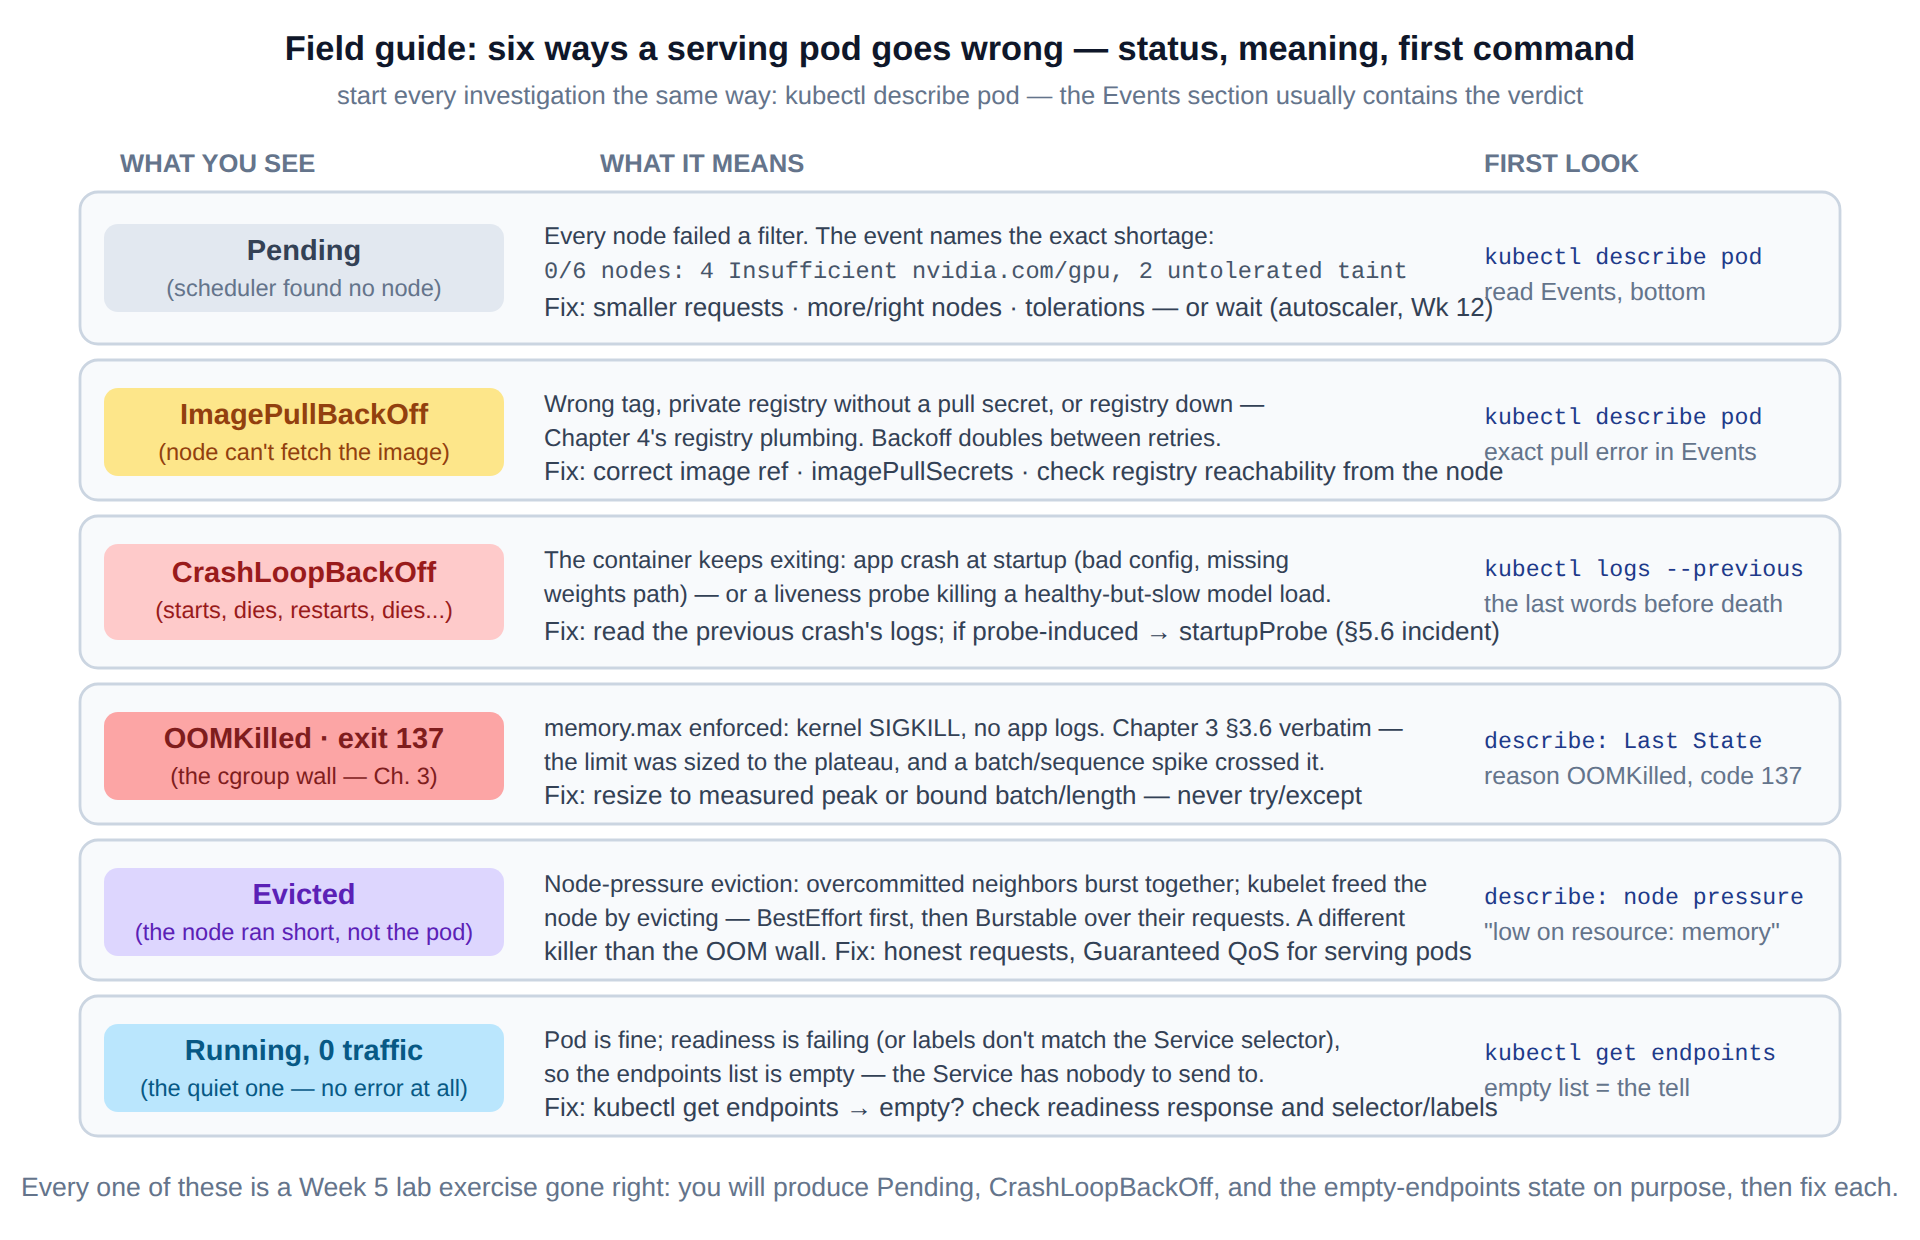
\includegraphics{figures/fig5-7_fieldguide.png}}\\[3pt]
  \figcaption{Figure 5-7  The six canonical failure states: what you see, what it means, where to look first. All six are staged deliberately in this week's lab.}
\end{tbbfigure}

\subsection*{The incident, end to end: CrashLoopBackOff on a healthy image}

The setup: a teammate ships \code{model-server:v9}, whose new model takes \textasciitilde{}90 seconds to load. It worked in \code{docker run}. On the cluster, the Deployment — whose author never set a startupProbe and left a brisk livenessProbe — produces this:

\begin{terminalbox}
\begin{Verbatim}[breaklines=true,breakanywhere=true,fontsize=\small,formatcom=\color{tbbtermfg},codes=\tbbcodeactive]
$ kubectl get pods
NAME                            READY   STATUS             RESTARTS   AGE
model-server-59f6c9d8b7-qv4tn   0/1     CrashLoopBackOff   5          8m
# five restarts in eight minutes. First reflex: describe, read Events.
$ kubectl describe pod model-server-59f6c9d8b7-qv4tn
...
Events:
  Warning  Unhealthy  Liveness probe failed: Get "http://10.244.1.61:8000
           /healthz": context deadline exceeded
  Normal   Killing    Container server failed liveness probe, will be
           restarted
  Normal   Pulled     Container image already present on machine
  Normal   Started    Started container server
# the kubelet is the killer - and it says so. Second reflex:
$ kubectl logs model-server-59f6c9d8b7-qv4tn --previous | tail -3
INFO  loading weights shard 5/8 ...
INFO  loading weights shard 6/8 ...
INFO  loading weights shard 7/8 ...
\end{Verbatim}
\end{terminalbox}
\figcaption{Transcript 5-9  The forensic chain: CrashLoopBackOff → describe names the liveness probe as the killer → logs --previous show a process guilty of nothing but loading slowly. No error appears anywhere, because nothing erred.}

Parse it like Chapter 3 taught you to parse the OOM chain. The \textbf{status} says the container keeps dying (\code{CrashLoopBackOff} is not a cause — it is the restart \textit{policy} backing off, doubling its delay between attempts). The \textbf{events} name the executioner: the kubelet, on behalf of a liveness probe that demanded an answer the server could not give while single-threadedly loading weights. The \textbf{previous logs} — the flight recorder; plain \code{logs} shows the \textit{current}, freshly-restarted attempt — end mid-load with no error at all. Kill, reload, kill: each restart re-pays the full load (Chapter 3's restart-loop economics), and the pod never once became Ready. The fix is the stanza from Transcript 5-3 — a startupProbe whose budget covers the worst-case load — after which the same image goes Ready in ninety quiet seconds. The general lesson outlives the incident: \textbf{in Kubernetes, the platform is one of your failure modes.} A probe, a limit, or an eviction can kill a healthy process, and the evidence lives in events, not in your application's logs.

\subsection*{Pending: the scheduler shows its work}

\begin{terminalbox}
\begin{Verbatim}[breaklines=true,breakanywhere=true,fontsize=\small,formatcom=\color{tbbtermfg},codes=\tbbcodeactive]
$ kubectl get pods
NAME                            READY   STATUS    RESTARTS   AGE
llm-server-7b9d5f4c66-x2jkp     0/1     Pending   0          3m
$ kubectl describe pod llm-server-7b9d5f4c66-x2jkp | tail -4
Events:
  Warning  FailedScheduling  0/6 nodes are available:
    4 Insufficient nvidia.com/gpu,
    2 node(s) had untolerated taint {team: batch}.
\end{Verbatim}
\end{terminalbox}
\figcaption{Transcript 5-10  Pending is the scheduler publishing its filter report (§5.5): six nodes, and the exact filter each failed. Nothing is wrong with the pod — the cluster cannot honor its constraints.}

Pending is the most self-documenting state in the system, because §5.5's filter phase writes its failure tally straight into the event: read it as \textit{"here is why each node was eliminated."} The remedies form a ladder — shrink the requests (does the pod really need 4 GPUs?), free or add capacity (Week 12's autoscaler automates exactly this), fix the addressing (tolerations, labels) — and one non-remedy worth naming: deleting and re-creating the pod, which re-runs the same filters against the same cluster and Pends again. Fix the constraint, not the symptom.

\subsection*{The other four, filed}

\begin{tbbitemize}
  \item \textbf{ImagePullBackOff} — the node cannot fetch the image: wrong tag, private registry without an \code{imagePullSecrets}, or registry unreachable from nodes. Chapter 4's registry plumbing; \code{describe} events contain the raw pull error. (A subtle serving variant: the tag exists but is 8 GB and the node disk is full — the event says so.)
  \item \textbf{OOMKilled / exit 137} — Chapter 3 §3.6, echoed by the platform: \code{describe} shows \code{Last State: Terminated, Reason: OOMKilled, Exit Code: 137}. Kubernetes adds one twist: \code{restartPolicy} resurrects the container with the \textit{same} limit, so an undersized limit becomes a crash-loop with a model-load cold start on every lap — §3.6's naive policy, now with a flywheel. The fix conversation is unchanged: resize to measured peak or bound the variable part; never try/except.
  \item \textbf{Evicted} — the \textit{node} ran short (Table 5-2): status \code{Evicted}, message "The node was low on resource: memory." The pod may have been innocent; QoS decided the victim. Chronic evictions mean dishonest requests somewhere on the node — audit the namespace, and move serving pods to Guaranteed.
  \item \textbf{Running but unrouted} — the quiet one, and the only state on this list with no error anywhere: the pod runs, liveness passes, but readiness never goes true (or labels do not match the Service selector), so the \textbf{endpoints list is empty} and the Service has nobody to send to. Clients see connection errors; every pod dashboard is green. The tell is one command — \code{kubectl get endpoints model-svc} — and the reflex of checking it is, in the author's experience, the single highest-value habit this chapter installs.
\end{tbbitemize}

\begin{calloutbox}{tbbpurple}{tbbpurplefill}
{\normalsize\bfseries\color{tbbpurple}The five reflexes (tape to your monitor)}\par\vspace{3pt}
\begin{tbbitemize}
  \item \code{kubectl describe pod <p>} — always first; Events hold the verdict (probes, scheduling, pulls, OOM, eviction).
  \item \code{kubectl logs <p> --previous} — the flight recorder: last words of the attempt that died, not the fresh one.
  \item \code{kubectl get endpoints <svc>} — silence with green dashboards = empty endpoints until proven otherwise.
  \item \code{kubectl exec -it <p> -- sh} — step inside (Chapter 3 told you this is setns) to test /ready by hand, inspect env and paths.
  \item \code{kubectl port-forward pod/\allowbreak <p> 8000:8000} — talk to one specific pod, bypassing the Service, to split "pod broken" from "routing broken."
\end{tbbitemize}
\end{calloutbox}

\vspace{3.0pt}

\begin{calloutbox}{tbbpurple}{tbbpurplefill}
{\normalsize\bfseries\color{tbbpurple}Think About It}\par\vspace{3pt}
\begin{tbbitemize}
  \item A container shows CrashLoopBackOff; logs --previous end cleanly; exit code is 137. Two different killers produce 137 (Chapter 3's SIGKILL arithmetic). Name both, and the exact describe fields that distinguish them.
  \item A team's readinessProbe checks the database dependency. A 30-second database blip makes every pod unready at once → endpoints empty → total outage, for a service that could have served cached answers. Argue for and against dependency-checking readiness probes, and propose the compromise.
  \item Design the sequence of commands to prove, in under a minute, that "the model server is fine; the Service selector is wrong." (port-forward and get endpoints are your friends.)
\end{tbbitemize}
\end{calloutbox}

\section{Lab: Your Model Server, Orchestrated}

This week's lab promotes Chapter 4's image from \code{docker run} to a managed fleet, then deliberately breaks it in every §5.6 way. Everything runs on a laptop: \code{minikube start --cpus 4 --memory 8g} (kind works identically); the course registry provides the image (a public fallback tag is in the handout). Budget note: no cloud spend required this week — the GPU transcripts of §5.5 are demonstration-only, and an optional appendix reproduces them on a managed cluster for teams that already have credits. Work inside a namespace: \code{kubectl create namespace ml}.

\subsection*{Part A — deploy, expose, and trust the loop}

Apply the Deployment of Transcript 5-3 and the Service of Transcript 5-6 (NodePort type on minikube). Verify the fleet with \code{get pods -o wide}, then re-run \textbf{Transcript 5-1's experiment on your own fleet}: delete a pod mid-curl-loop and capture the reconciliation. Then perform a rolling update to \code{:v8} while a terminal runs a one-request-per-second curl loop against the Service — the deliverable's money shot is that loop's output across the entire rollout: \textbf{zero failed requests}, because readiness gates the pace while your Chapter 3 SIGTERM handler drains the old pods. (Then break it on purpose: remove the readinessProbe, roll to \code{:v9-slow}, and watch the same curl loop error — the negative control that proves what readiness was buying you.)

\subsection*{Part B — the translation, verified by hand}

Reproduce Transcript 5-7 yourself: \code{minikube ssh}, walk the cgroup tree under \code{/\allowbreak sys/\allowbreak fs/\allowbreak cgroup/\allowbreak kubepods.slice/\allowbreak }, and photograph your YAML numbers sitting in \code{memory.max} and \code{cpu.max} — the chapter's thesis, in your own terminal. Then stage the OOM: set \code{limits.memory: 256Mi} on the standard model, apply, and collect the Kubernetes-flavored evidence chain — \code{describe} showing \code{OOMKilled /\allowbreak  137}, plus the restart counter climbing as the crash-loop pays the model-load cold start on every lap. Restore honest limits, and note the before/after in your report with §3.6's vocabulary.

\subsection*{Part C — break it, diagnose it, fix it}

Three staged incidents, each ending with the fix applied and one sentence naming the section that predicted it. \textbf{(1) Pending:} request \code{nvidia.com/\allowbreak gpu: 1} on your GPU-less minikube; capture the FailedScheduling event and read the filter report aloud (§5.5); fix by removing the request. \textbf{(2) The probe incident:} set env \code{SLOW\_LOAD=90} (the course image simulates a slow model load), delete the startupProbe, tighten liveness to \code{periodSeconds: 5, failureThreshold: 2}; reproduce Transcript 5-9's full forensic chain — status, events, \code{logs --previous}; fix with the startupProbe stanza and show the same image going Ready. \textbf{(3) The quiet failure:} change the readiness path to \code{/\allowbreak readyz} (a typo the server does not serve); observe Running pods, green liveness, empty \code{get endpoints}, and failing client curls; fix and watch the endpoints repopulate.

\begin{calloutbox}{tbbpurple}{tbbpurplefill}
{\normalsize\bfseries\color{tbbpurple}Lab checklist}\par\vspace{3pt}
\begin{tbbitemize}
  \item Part A artifacts: \code{get pods -o wide} of the fleet · the delete-and-reconcile capture · the uninterrupted curl loop across a rolling update · the negative control (no readiness → errors).
  \item Part B artifacts: node-side \code{memory.max} and \code{cpu.max} matching your YAML · the OOMKilled describe block with restart count · restored config.
  \item Part C artifacts: the FailedScheduling filter report · Transcript 5-9 reproduced (events + logs --previous) + the fix going Ready · the empty-endpoints tell and its repopulation.
  \item Report: one page, three observations, each naming its section (e.g., "the liveness kill left no application log — §5.6's platform-as-failure-mode").
  \item Cleanup: \code{kubectl delete namespace ml}; \code{minikube stop}. (No cloud meter this week — the habit stays anyway.)
\end{tbbitemize}
\end{calloutbox}

\vspace{3.0pt}

\begin{calloutbox}{tbbpurple}{tbbpurplefill}
{\normalsize\bfseries\color{tbbpurple}Think About It}\par\vspace{3pt}
\begin{tbbitemize}
  \item During Part A's rolling update, the curl loop never failed. Enumerate every mechanism that had to cooperate — from readiness gating and endpoints updates down to Chapter 3's SIGTERM handler — and identify which single removal breaks the guarantee most cheaply.
  \item minikube is one node. Name three lab behaviors that would differ on a real five-node cluster, and one §5.6 state that a single-node cluster can never produce authentically.
\end{tbbitemize}
\end{calloutbox}

\namedsection{Summary}{The Chapter in Ten Points}

\qitem{1}{\textbf{Kubernetes is a reconciliation loop}: desired state in etcd, controllers that observe, diff, and act — forever. You declare nouns; the verbs are emergent. A deleted pod is not an event anyone handles; it is drift, and drift gets corrected.}

\qitem{2}{\textbf{Declarative invariants beat imperative instructions} because they do not decay: node failures, fat-fingered deletions, and deploys are all the same thing to the loop. Autoscaling (Wk 12) and CI/CD (Wk 13) are just additional writers of desired state.}

\qitem{3}{\textbf{The anatomy is a database with opinions}: API server (the only door), etcd (the only state), scheduler (the matchmaker), controller manager (the loops), kubelet (the hands), kube-proxy (the NAT). Components never call each other — everything is watches on the API server, which is why any piece can die without taking the system down.}

\qitem{4}{\textbf{Nothing named Kubernetes runs your container.} The chain is apply → objects → scheduler binds → kubelet → CRI → containerd → runc → Chapter 3's namespaces and cgroups. The kubelet is the ghostwriter that finally writes memory.max.}

\qitem{5}{\textbf{A pod is the unit of scheduling and sharing}: containers joined to a pause container's NET namespace (one IP, localhost sidecars) plus shared volumes; MNT and PID stay private. Pods are mortal and label-addressed — never target their IPs. The workload shape all of this assumes is the \textbf{microservice} — one capability per service, code complexity traded for operational complexity; the trinity is that trade's starter kit, and one microservice = one Deployment + one Service.}

\qitem{6}{\textbf{Probes are three different questions}: startup ("finished booting?") covers the model load; readiness ("may I send traffic?") controls Service endpoints and paces rollouts; liveness ("alive at all?") restarts. Confuse liveness with readiness under a 90-second model load and a healthy image crash-loops forever.}

\qitem{7}{\textbf{Deployments make rollouts bloodless mechanically}: one ReplicaSet per template version, maxSurge/maxUnavailable pacing, readiness as the gate, rollback as repointing. Every Terminating pod replays Chapter 3's SIGTERM tape — your handler does the draining; Kubernetes only schedules it.}

\qitem{8}{\textbf{requests are scheduler arithmetic; limits are cgroup walls.} requests.cpu also seeds cpu.weight (soft, work-conserving); limits become cpu.max (burst throttling — §3.3's manufactured p99) and memory.max (§3.6's OOM wall). The requests/limits gap is deliberate overcommit; when the bet loses, the kubelet evicts — a second killer with a different signature (Evicted vs. OOMKilled/137). QoS classes (Guaranteed / Burstable / BestEffort) set oom\_score\_adj: serving pods run Guaranteed.}

\qitem{9}{\textbf{GPUs schedule as integer extended resources — no fractions, no overcommit, requests = limits — because no cgroup controller referees GPU sharing (Ch. 3's negative space).} Taints repel, affinity aims, device plugins advertise and allocate. Bin-pack GPU fleets: fragmentation is Pending with money attached, and stranded GPUs bill idle. Fractions come from Ch. 2's MIG/time-slicing (Wk 12).}

\qitem{10}{\textbf{Six states cover nearly every serving incident}: Pending (read the filter report), ImagePullBackOff (Ch. 4 plumbing), CrashLoopBackOff (app crash or probe kill — logs --previous), OOMKilled/137 (Ch. 3 verbatim), Evicted (node pressure), and Running-but-unrouted (empty endpoints — the quiet one). describe → events is the front door; the platform itself is one of your failure modes.}

\namedsection{Exercises}{}

\subsection*{A. Multiple choice}

\qitem{1}{You delete one pod of a three-replica Deployment. What happens, and via which mechanism?}

\begin{tbboptions}
  \item ① Nothing — pods are only recreated at the next deploy
  \item ② The kubelet restarts the same pod because restartPolicy is Always
  \item ③ The ReplicaSet controller observes desired 3 ≠ actual 2 and creates a new pod (new name, possibly a new node)
  \item ④ kube-proxy recreates it from the Service's endpoints cache
\end{tbboptions}

\qitem{2}{Which component causes limits.memory: 1.75Gi to become a memory.max file on a node?}

\begin{tbboptions}
  \item ① The API server, when validating the manifest
  \item ② The scheduler, at bind time
  \item ③ etcd, via a storage hook
  \item ④ The node's kubelet, driving the container runtime over CRI
\end{tbboptions}

\qitem{3}{Which statement about requests and limits is correct?}

\begin{tbboptions}
  \item ① requests are enforced by cpu.max; limits are advisory
  \item ② requests feed scheduler placement (and cpu.weight); limits become cgroup walls enforced at runtime
  \item ③ Both are enforced identically; requests are simply the minimum
  \item ④ limits affect only GPUs
\end{tbboptions}

\qitem{4}{A pod is Running, liveness passes, but clients get connection errors through the Service. The highest-yield first check is:}

\begin{tbboptions}
  \item ① kubectl logs — look for stack traces
  \item ② Restart the Deployment
  \item ③ kubectl get endpoints — an empty list means readiness (or the selector) is the problem
  \item ④ Reboot the node
\end{tbboptions}

\qitem{5}{A container sets requests = limits for memory only; its CPU request is below its CPU limit. Its QoS class is:}

\begin{tbboptions}
  \item ① Guaranteed — memory is what matters
  \item ② Burstable — Guaranteed requires requests = limits for both CPU and memory in every container
  \item ③ BestEffort — CPU decides the class
  \item ④ It depends on the node's allocatable
\end{tbboptions}

\qitem{6}{A 1-GPU pod stays Pending. describe shows: "0/6 nodes are available: 4 Insufficient nvidia.com/gpu, 2 node(s) had untolerated taint \{nvidia.com/gpu: present\}." Two nodes in fact have free GPUs. The correct fix is:}

\begin{tbboptions}
  \item ① Increase the pod's CPU requests so it outbids other pods
  \item ② Add the matching toleration to the pod so the two tainted GPU nodes pass filtering
  \item ③ Set nvidia.com/gpu: 0.5 to fit more easily
  \item ④ Delete and recreate the pod to re-run scheduling
\end{tbboptions}

\subsection*{B. Short answer}

\qitem{1}{Trace kubectl apply of a new 3-replica Deployment to running containers in five steps, naming the component responsible for each step.}

\qitem{2}{Why is Σ limits > allocatable permitted on a node while Σ requests > allocatable is impossible — and name the two backstops that handle the case where the overcommit bet loses.}

\qitem{3}{Write plausible probe stanzas (probe type, period, failureThreshold) for a server whose model load takes up to 120 seconds, and justify each number in one clause.}

\qitem{4}{OOMKilled versus Evicted: give trigger, executioner, and the one-line signature of each.}

\subsection*{C. Essay}

\qitem{1}{"Never set CPU limits on latency-critical serving pods." Argue for and against, using §3.3's throttling arithmetic, cpu.weight's work-conserving behavior, the Guaranteed-QoS requirement, and platform-governance realities. State your recommendation for the course project's model server and defend it.}

\qitem{2}{Design node pools, labels, taints, QoS choices, and a packing policy for one cluster serving: (a) a latency-critical quantized model on T4s, (b) a nightly batch-scoring job that wants A100s, and (c) ordinary CPU microservices. Justify each choice with a failure or cost scenario it prevents, and identify what Week 12's autoscaler adds to your design.}

\qitem{3}{"Self-healing hides root causes: a reconciliation loop that silently replaces crashing pods is an incident-suppression system, not an incident-resolution system." Discuss, drawing on the restart-loop economics of model loading (§3.6, §5.6), the observability surfaces of §5.6, and what a mature team must add (Wk 14) so that convergence and diagnosis coexist.}

\namedsection{Answers and Commentary}{}

\subsection*{A. Multiple choice}

\qitem{1}{\textbf{③} Reconciliation, not resurrection: the ReplicaSet loop counts 2 ≠ 3 and creates a fresh pod (new suffix, new IP, possibly a new node). ② confuses container restarts within a pod with pod replacement. (§5.1)}

\qitem{2}{\textbf{④} The kubelet is the hands — and the ghostwriter: it drives containerd/runc over CRI, which write the cgroup files. The API server stores, the scheduler places; neither touches a node. (§5.2, §5.4)}

\qitem{3}{\textbf{②} The chapter's central asymmetry: requests are planning numbers (never enforced at runtime; cpu request also seeds cpu.weight); limits are Chapter 3's cgroup walls, enforced every millisecond. (§5.4)}

\qitem{4}{\textbf{③} Running-but-unrouted is the quiet failure: liveness green, readiness failing (or labels not matching the selector) → empty endpoints → the Service has nobody. Logs (①) show nothing because nothing erred. (§5.3, §5.6)}

\qitem{5}{\textbf{②} Guaranteed is strict: requests = limits for \textit{both} resources, \textit{every} container. Partial equality is Burstable — a common and reasonable serving compromise (memory-Guaranteed), but not the class name. (§5.4)}

\qitem{6}{\textbf{②} Read the filter report: four nodes lack free GPUs; two have them but are tainted and the pod lacks the toleration. Tolerations unlock the tainted pair. ③ is illegal (integers only); ④ re-runs the same filters to the same verdict. (§5.5, §5.6)}

\subsection*{B. Short answer}

\qitem{1}{(1) API server validates and persists the Deployment (etcd). (2) Deployment controller creates a ReplicaSet; ReplicaSet controller creates 3 Pod objects with empty nodeName. (3) Scheduler filters/scores/binds each pod to a node. (4) Each node's kubelet pulls the image and drives containerd → runc: namespaces, cgroups, overlayfs. (5) Kubelet reports status; probes pass; endpoints admit the pods. (§5.2)}

\qitem{2}{The scheduler only ever accounts requests, so placement can never oversubscribe them; limits are burst ceilings deliberately allowed to sum past the node (overcommit-as-feature — everyone may burst, rarely together). Backstops when the bet loses: per-container cgroup walls (memory.max → OOMKilled/137) and kubelet node-pressure eviction (QoS-ordered, status Evicted). (§5.4)}

\qitem{3}{startupProbe: httpGet /healthz, periodSeconds 5, failureThreshold ≥ 30 (5 × 30 = 150 s > 120 s worst load, with margin) — holds the other probes off. readinessProbe: /ready, period 5, threshold 2–3 — fast traffic gating. livenessProbe: /healthz, period 10–15, threshold 3 — lazy on purpose; it restarts only true deadlock. (§5.3, §5.6)}

\qitem{4}{OOMKilled: this container crossed its own memory.max; kernel OOM killer SIGKILLs; signature Last State: OOMKilled, exit 137 (+ dmesg). Evicted: the node ran short under overcommit; the kubelet terminates chosen victims by QoS/usage-over-request; signature status Evicted, "The node was low on resource: memory." (§5.4, §5.6)}

\subsection*{C. Essay (grading points)}

\qitem{1}{For "never limit": §3.3 arithmetic (30 ms of work → 110–190 ms under a 0.2-CPU cap; p99 spikes; profiler-blind), cpu.weight already guarantees fairness under contention while wasting nothing, idle headroom is cheap insurance. Against: runaway protection and billing hygiene at platform scale; multi-tenant fairness against pods with dishonest requests; Guaranteed QoS requires limits — and Guaranteed's oom protection matters on overcommitted nodes; static CPU-manager pinning needs integer requests = limits. Full credit engages the tension and lands a position: e.g., generous requests = limits (Guaranteed) sized above measured peak CPU, or no CPU limit + memory-Guaranteed Burstable with a PriorityClass, each with its stated trade. (§5.4)}

\qitem{2}{Look for: three pools (t4-serving, a100-batch, cpu-general) with labels gpu=t4/a100; taints on both GPU pools so CPU riffraff never lands (§5.5); model A pods with toleration + affinity gpu=t4, Guaranteed QoS; batch B tolerating a100 pool with low PriorityClass (evictable) and no CPU limits; bin-packing (MostAllocated) scoring on GPU pools for scale-down and multi-GPU headroom; honest CPU requests on GPU pods to avoid stranding. Cost scenarios: fragmentation → forced node add; stranded GPUs behind CPU-hungry daemonsets; batch preempting latency pods (prevented by priority + taints). Wk 12: autoscaler deletes bin-packed empty nodes; scale-to-zero for the batch pool. (§5.4–5.5)}

\qitem{3}{Strong answers grant the premise its evidence — a crash-looping model server that self-heals every 90 s can hide an undersized limit for weeks while paying cold-start latency at every lap (§3.6's flywheel), and Transcript 5-9's incident produces no app-log evidence at all — then rebut: convergence is what makes 3 a.m. survivable; the loop \textit{localizes} rather than hides evidence (restart counters, events, Last State, memory.events), you just have to look at the platform's surfaces, not the app's. Mature practice (Wk 14): alert on restart counts, oom\_kill counters, endpoints emptiness, rollout stalls — i.e., alert on drift-correction \textit{frequency}, not just availability. Conclusion worth rewarding: reconciliation without observability is incident suppression; with it, it is incident \textit{buffering} — time bought for diagnosis. (§5.1, §5.6)}

\namedsection{Further Reading}{}

Entries tagged \textbf{[This week]} are required reading now; a \textbf{[Wk N]} tag marks material that pays off in that later week.

\begin{tbbitemize}
  \item \textbf{[This week] Kubernetes docs: Concepts → "Pods", "Deployments", "Service"} — the canonical descriptions behind §5.3. Read the Concepts pages, not the task pages: concepts explain the \textit{why} that tutorials skip.
  \item \textbf{[This week] Kubernetes docs: "Pod Lifecycle"} (including probes) — the authoritative source for §5.3's three questions, container states, and restart backoff; the CrashLoopBackOff mechanics of §5.6 are all here.
  \item \textbf{[This week] Kubernetes docs: "Resource Management for Pods and Containers" + "Configure Quality of Service for Pods"} — §5.4's primary sources: requests vs. limits, allocatable, QoS classes, and (in the node docs) node-pressure eviction ordering.
  \item \textbf{Kelsey Hightower, "Kubernetes the Hard Way" (GitHub)} — build a cluster once with no installer, and §5.2's anatomy stops being a diagram. Do it in a rainy weekend, once, ever; the mental model lasts a career.
  \item \textbf{Marko Lukša, "Kubernetes in Action" (2nd ed., Manning)} — the best book-length treatment; chapters on pods, Deployments, Services, and resource management map one-to-one onto §5.3–5.4 with more API surface.
  \item \textbf{Verma et al., "Large-scale cluster management at Google with Borg" (EuroSys 2015)} — where the ideas come from: declarative jobs, reconciliation, bin-packing, and the utilization economics that §5.5 inherits. Read §5 (utilization) with Chapter 1's cost lens.
  \item \textbf{[Wk 6] Kubernetes docs: "Ingress" and cloud provider load-balancer docs} — the layer Week 6 adds in front of your Service (API gateway, TLS, routing).
  \item \textbf{[Wk 12] NVIDIA GPU Operator and device-plugin docs (time-slicing, MIG strategies); Kubernetes Cluster Autoscaler FAQ; HPA/KEDA docs} — the operational continuation of §5.5: fractional GPUs, scale-up on Pending, scale-down of bin-packed empties, and event-driven autoscaling.
  \item \textbf{[Wk 13] Argo Rollouts documentation (canary, blue-green)} — what Deployments' rolling update grows into when Week 13 adds progressive delivery and automated analysis.
\end{tbbitemize}

\vspace{5.0pt}

\begin{calloutbox}{tbbblue}{tbbbluefill}
{\normalsize\bfseries\color{tbbblue}Next chapter — Chapter 6: Storage and Networking}\par\vspace{3pt}
Your model server now runs as a fleet with a stable name — but its weights are still baked into the image (Chapter 3 warned you), and its Service is still cluster-internal plumbing. Next week completes the serving skeleton: \textbf{block versus object storage} and why model weights live in an object store; the \textbf{model-store pattern} — weights and datasets on S3-compatible storage, loaded at startup, versioned independently of images (the Week 6 lab builds exactly this path and Week 13's registry story depends on it); and the front door — \textbf{load balancers and API gateways} in front of your Service, plus enough \textbf{VPC and security-group} literacy to keep an expensive GPU fleet off the public internet. After Week 6, the infrastructure half of the course is complete — and Part 2 starts serving models on top of it.
\end{calloutbox}
